\documentclass[a4paper]{article}

\IfFileExists{ctex.sty}{
  \usepackage[fontset=fandol]{ctex}
}{
  \usepackage{fontspec}
  \XeTeXlinebreaklocale "zh"
  \XeTeXlinebreakskip = 0pt plus 1pt
  \IfFontExistsTF{Songti SC}{\setmainfont{Songti SC}}{}
  \IfFontExistsTF{Heiti SC}{\setsansfont{Heiti SC}}{}
}

\usepackage{amsmath, amssymb}
\usepackage{graphicx}
\usepackage[margin=2.5cm]{geometry}
\usepackage[most]{tcolorbox}
\usepackage{etoolbox}
\usepackage{listings}
\usepackage{hyperref}
\usepackage{booktabs}
\usepackage{subcaption}
\usepackage{float}
\usepackage{tikz}

\newtcolorbox{knowledgebox}[1]{
    enhanced, colback=blue!5!white, colframe=blue!75!black, colbacktitle=blue!75!black,
    coltitle=white, fonttitle=\bfseries, title=#1, attach boxed title to top left={yshift=-2mm, xshift=2mm},
    boxrule=1pt, sharp corners
}
\newtcolorbox{importantbox}[1]{
    enhanced, colback=yellow!10!white, colframe=yellow!80!black, colbacktitle=yellow!80!black,
    coltitle=black, fonttitle=\bfseries, title=#1, sharp corners
}
\newtcolorbox{warningbox}[1]{
    enhanced, colback=red!5!white, colframe=red!75!black, colbacktitle=red!75!black,
    coltitle=white, fonttitle=\bfseries, title=#1, sharp corners
}

\lstset{
    basicstyle=\ttfamily\small,
    keywordstyle=\color{blue},
    stringstyle=\color{red!60!black},
    commentstyle=\color{green!60!black},
    breaklines=true,
    frame=single,
    numbers=left,
    numberstyle=\tiny\color{gray},
    captionpos=b,
    extendedchars=false
}

\newcommand{\vtag}{\protect\footnotemark}
\newcommand{\srcnote}[1]{\footnotetext{视频画面时间区间：#1。}}

\newcommand{\notetitle}{工具调用：从 token 预测到真实动作}
\newcommand{\notesubtitle}{CMU 11-768《AI Agents》第 2 讲：Tool Use for Language Model Agents}
\newcommand{\noteauthors}{lecture-to-notes 整理}
\newcommand{\notedate}{\today}
\newcommand{\videochannel}{Graham Neubig（CMU 11-768 AI Agents）}
\newcommand{\videopublishdate}{2026-09-08}
\newcommand{\videoduration}{57 分 22 秒}
\newcommand{\videourl}{https://www.youtube.com/watch?v=jXChFB4JSyw}
\newcommand{\videocoverpath}{cover.jpg}

\begin{document}

\begin{titlepage}
\centering
{\Large 课程笔记\par}
\vspace{1.2cm}
{\huge\bfseries \notetitle\par}
\vspace{0.3cm}
{\large \notesubtitle\par}
\vspace{0.5cm}
{\large \noteauthors\par}
\vspace{0.3cm}
{\large \notedate\par}
\vspace{1.0cm}

\includegraphics[width=0.82\textwidth,height=0.40\textheight,keepaspectratio]{\videocoverpath}\par

\vfill
\begin{tcolorbox}[width=0.9\textwidth, colback=black!2!white, colframe=black!60, sharp corners]
\textbf{视频作者/频道}：\videochannel\par
\textbf{发布日期}：\videopublishdate\par
\textbf{视频时长}：\videoduration\par
\textbf{视频链接}：\href{\videourl}{\nolinkurl{\videourl}}
\end{tcolorbox}
\end{titlepage}

\tableofcontents
\newpage

%% --- 正文内容开始 --- %%

\section{工具是什么：让语言模型动手}

\subsection*{本节回答的问题}
工具在 agent 系统里处于什么位置？它给语言模型带来的价值可以分成哪几类，什么时候才值得调用？

\subsection{定义：模型提议，系统执行}

这讲的第一句话就把工具的定位说清了：\textbf{工具是语言模型调用外部计算机程序的接口}。语言模型本身只是 token 预测器，它无法查今天的天气、无法上网、无法真的运行一段代码；工具把"预测出一段文本"变成"对一个外部程序发起一次调用"。幻灯片列举的典型例子是 Python 解释器、搜索引擎、计算器、各类 API 与浏览器，并给出一句关键的分工描述：

\begin{figure}[H]
\centering
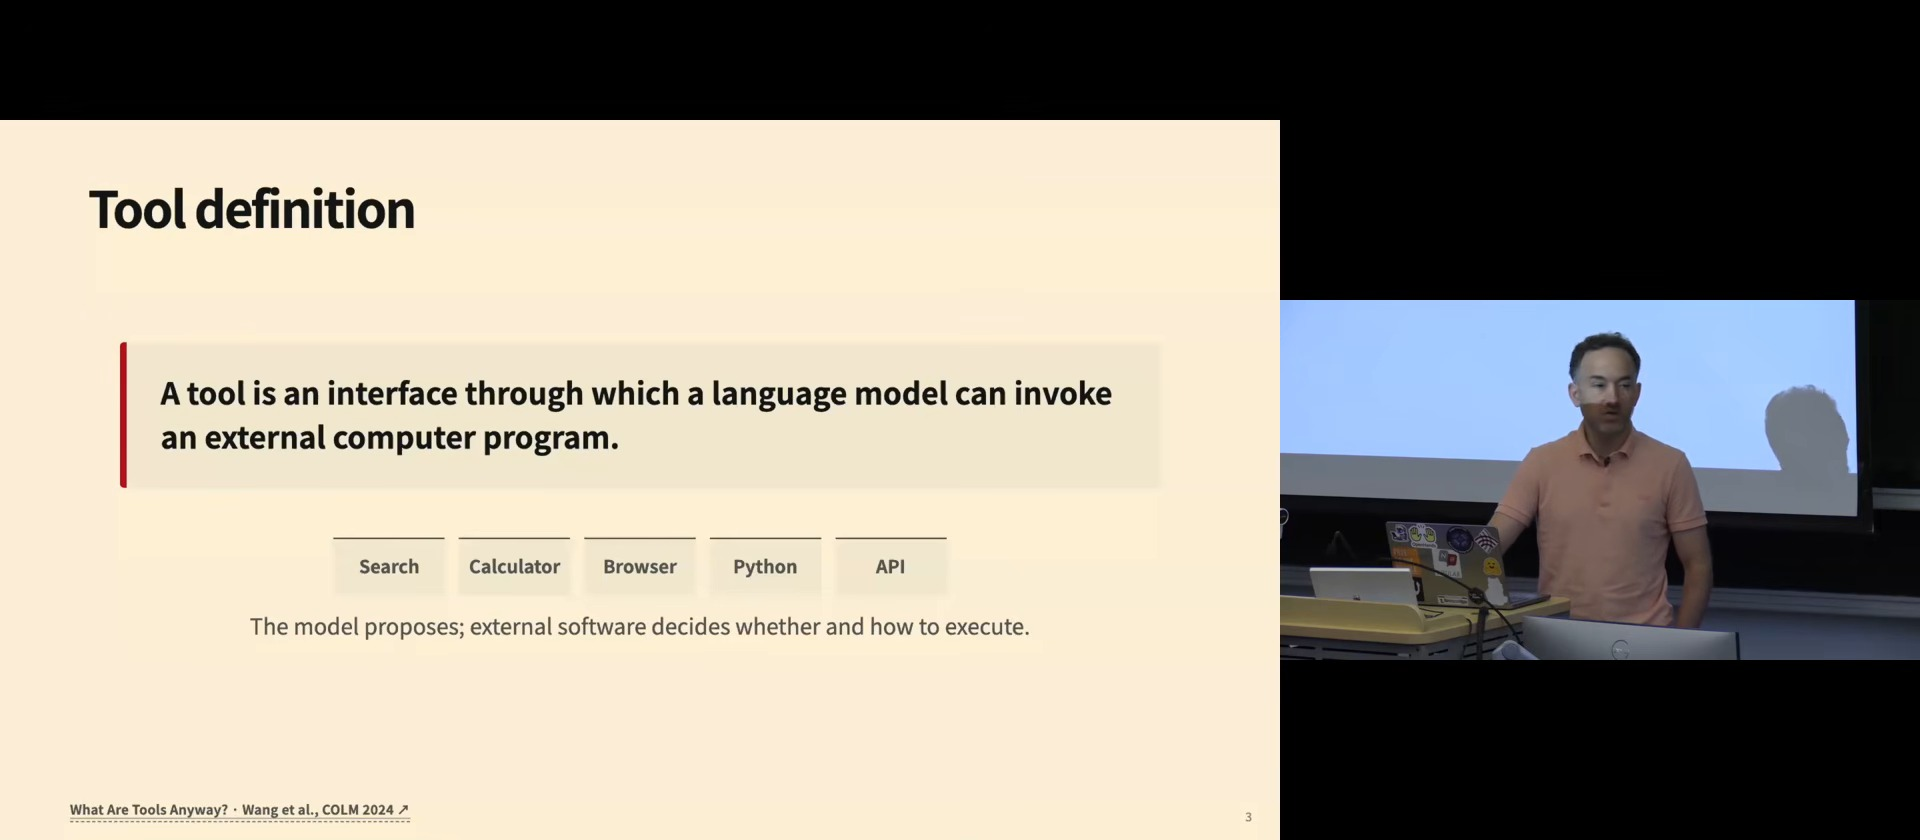
\includegraphics[width=\textwidth]{figures/fig_01_tool_definition.jpg}
\caption{工具的定义：模型调用外部程序的接口——"The model proposes; external software decides whether and how to execute"\vtag}
\end{figure}
\srcnote{00:00:45--00:00:59}

\begin{importantbox}{工具不是一个动作，而是一条接口}
模型能做的是"提出调用"；是否执行、以什么权限执行、执行结果如何裁剪，全部属于 harness 与外部软件的职责。把这条边界记住，后面关于校验、沙箱、凭证隔离的讨论都会变得自然。
\end{importantbox}

\subsection{两类价值：扩展能力与降低难度}

工具的价值被分成两类，这个区分决定了后面所有的设计取舍。

第一类是\textbf{扩展（extend）}：做模型根本做不到的事——获取它参数字典里不存在的信息（当前时间、今天的网页），或者作用于模型碰不到的状态（改文件、下单、发消息）。第二类是\textbf{促进（facilitate）}：事情模型其实能做，只是用工具更划算——比如乘法，模型现在算得不错，但做七位数乘法要一步步推理，而计算器一瞬间就给出答案。

\begin{figure}[H]
\centering
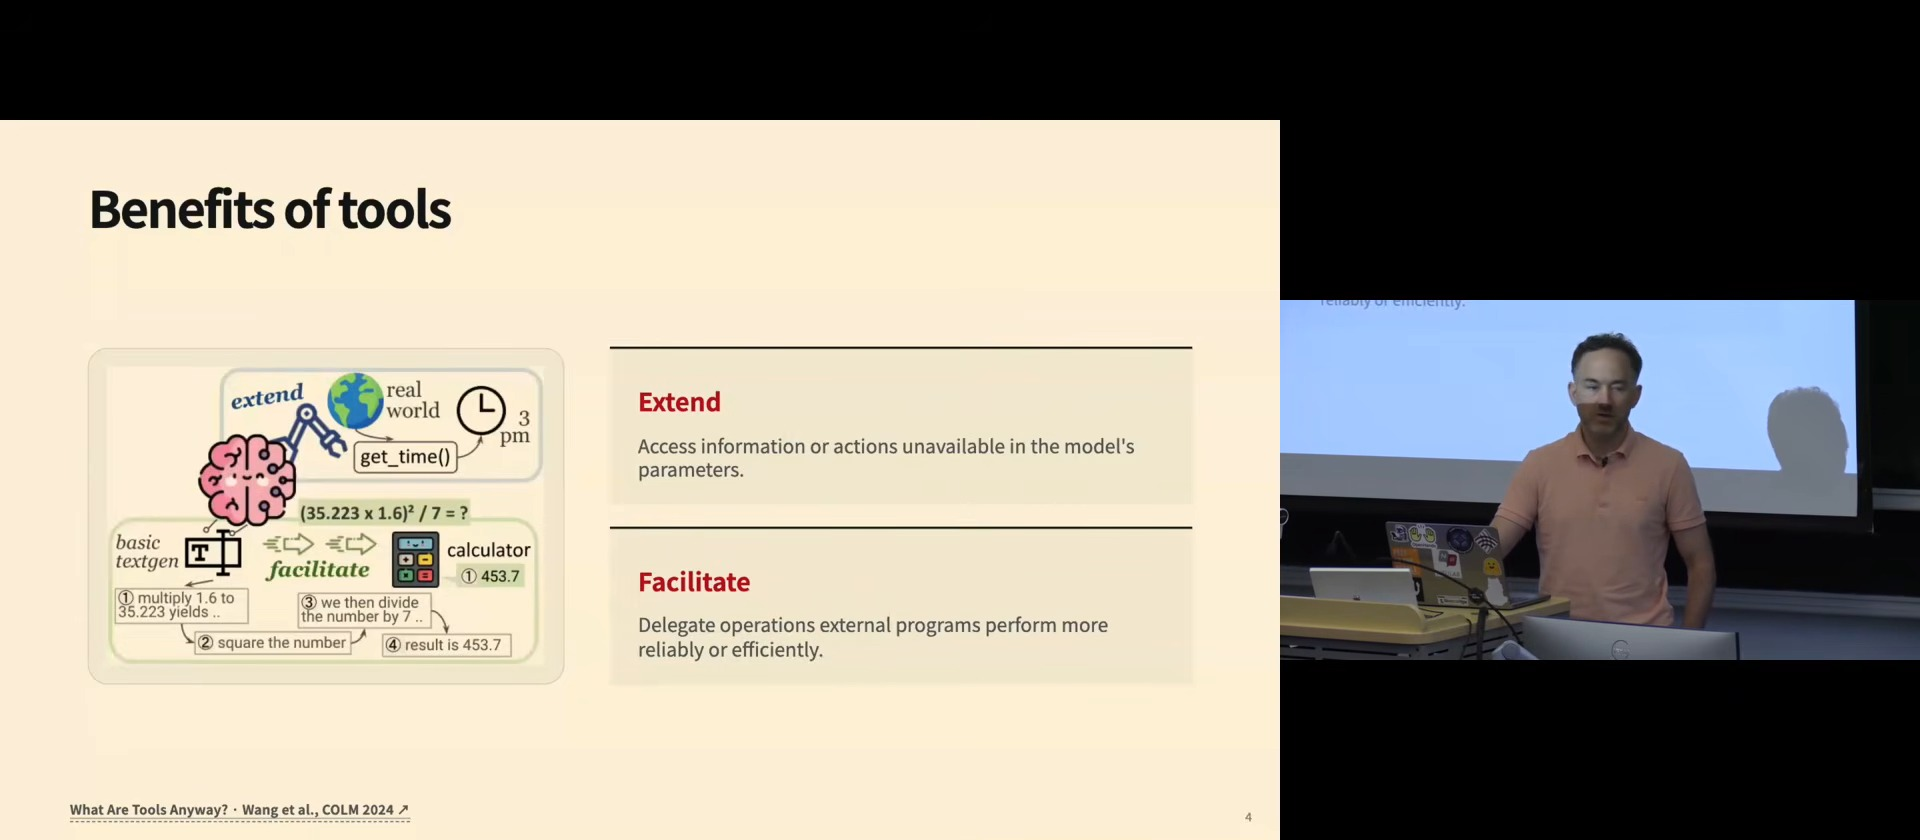
\includegraphics[width=\textwidth]{figures/fig_02_benefits.jpg}
\caption{两类收益：extend 是"参数里没有的信息或动作"，facilitate 是"能做但更慢更笨"（例：get\_time 与计算器）\vtag}
\end{figure}
\srcnote{00:01:45--00:01:59}

第二类里最值得记住的例子是幻灯片上那个算式 $\frac{35.223 \times 1.6}{7}$：模型可以"一步步算"并给出一个看起来合理的答案，但每一步都可能出错；调用计算器则把这个问题从"推理任务"降级成"工具调用 + 读结果"。

第三张表把"需求—工具—收益"三列摆在一起：需要当前信息 → 用搜索 → 得到新鲜证据；需要精确计算 → 用计算器或 Python → 得到可靠执行；需要私有状态 → 用账户类 API → 得到个性化结果；需要改变外部世界 → 用浏览器或业务 API → 让动作真的发生。讲者给出一条判据——\textbf{只有当收益盖过延迟、成本、失败风险时，才值得调用工具}。

\begin{figure}[H]
\centering
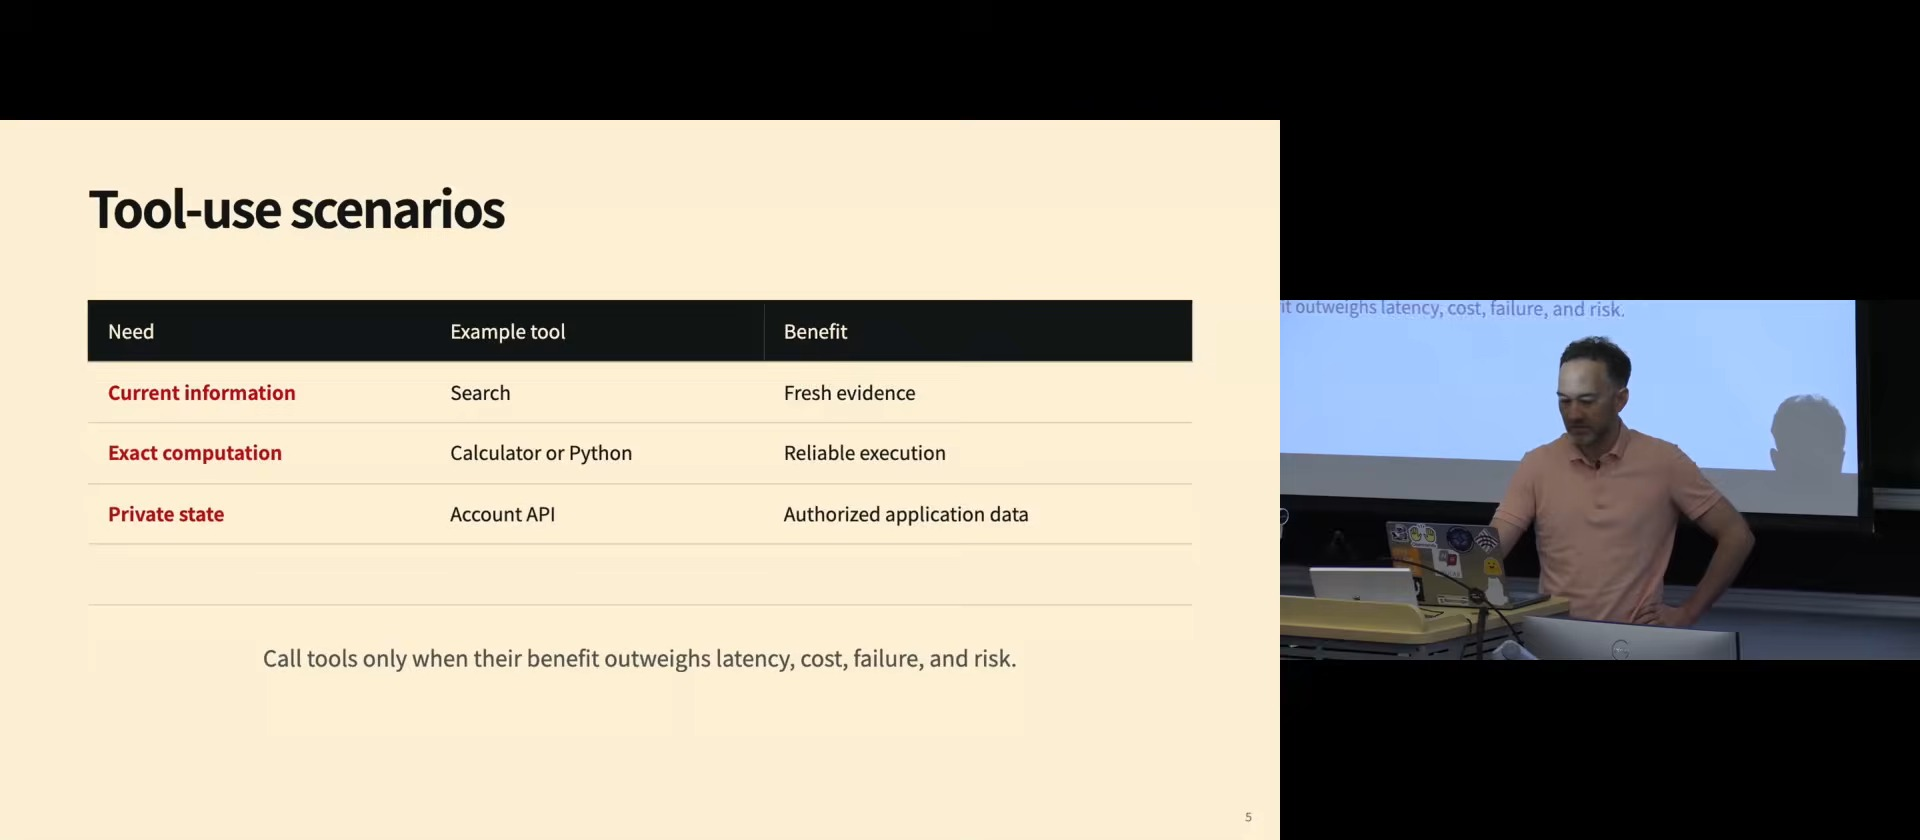
\includegraphics[width=\textwidth]{figures/fig_03_scenarios.jpg}
\caption{工具使用场景表：需求、示例工具与收益；调用与否取决于收益是否盖过延迟、成本、失败与风险\vtag}
\end{figure}
\srcnote{00:03:15--00:03:29}

课堂上有人问 ChatGPT 现在能做什么，回答涵盖了写代码、渲染 Blender 场景、生成图片、联网搜索商品、编译 LaTeX 生成 PDF、发 Slack 消息。讲者由此给出一个设计方法：\textbf{从"我们希望它具备的能力"出发，为每项能力定义一个窄接口}，而不是先攒一堆 API 再想怎么用。

\begin{knowledgebox}{"RAG 已死"是个误会}
讲者顺带回应了"retrieval-augmented generation 已经过时"的说法："检索上下文再作答"这件事已经变成默认做法，普遍到人们不再意识到自己在用它——\textbf{它不是死了，而是活成了基础设施}。这条判断对读者有用：判断一项技术是否过时，看它是否还出现在产品里，而不是看它是否还被单独讨论。
\end{knowledgebox}

\subsection{工具的分类与实例}

课程给出一组"典型工具"，并说明绝大多数现实工具都能归入其中。每一类都配了完整的调用链路（用户问题 → 模型提出的调用 → 工具 → 返回值 → 自然语言回复）。

\textbf{文本回复}是最朴素的一类：模型回答"加纳的首都是哪里"，调用 \texttt{finish("Accra is the capital of Ghana.")} 结束循环。这里的 \texttt{finish} 是 harness 的控制动作，不是外部工具——它的作用是让循环停下来并交出最终文本。

\begin{figure}[H]
\centering
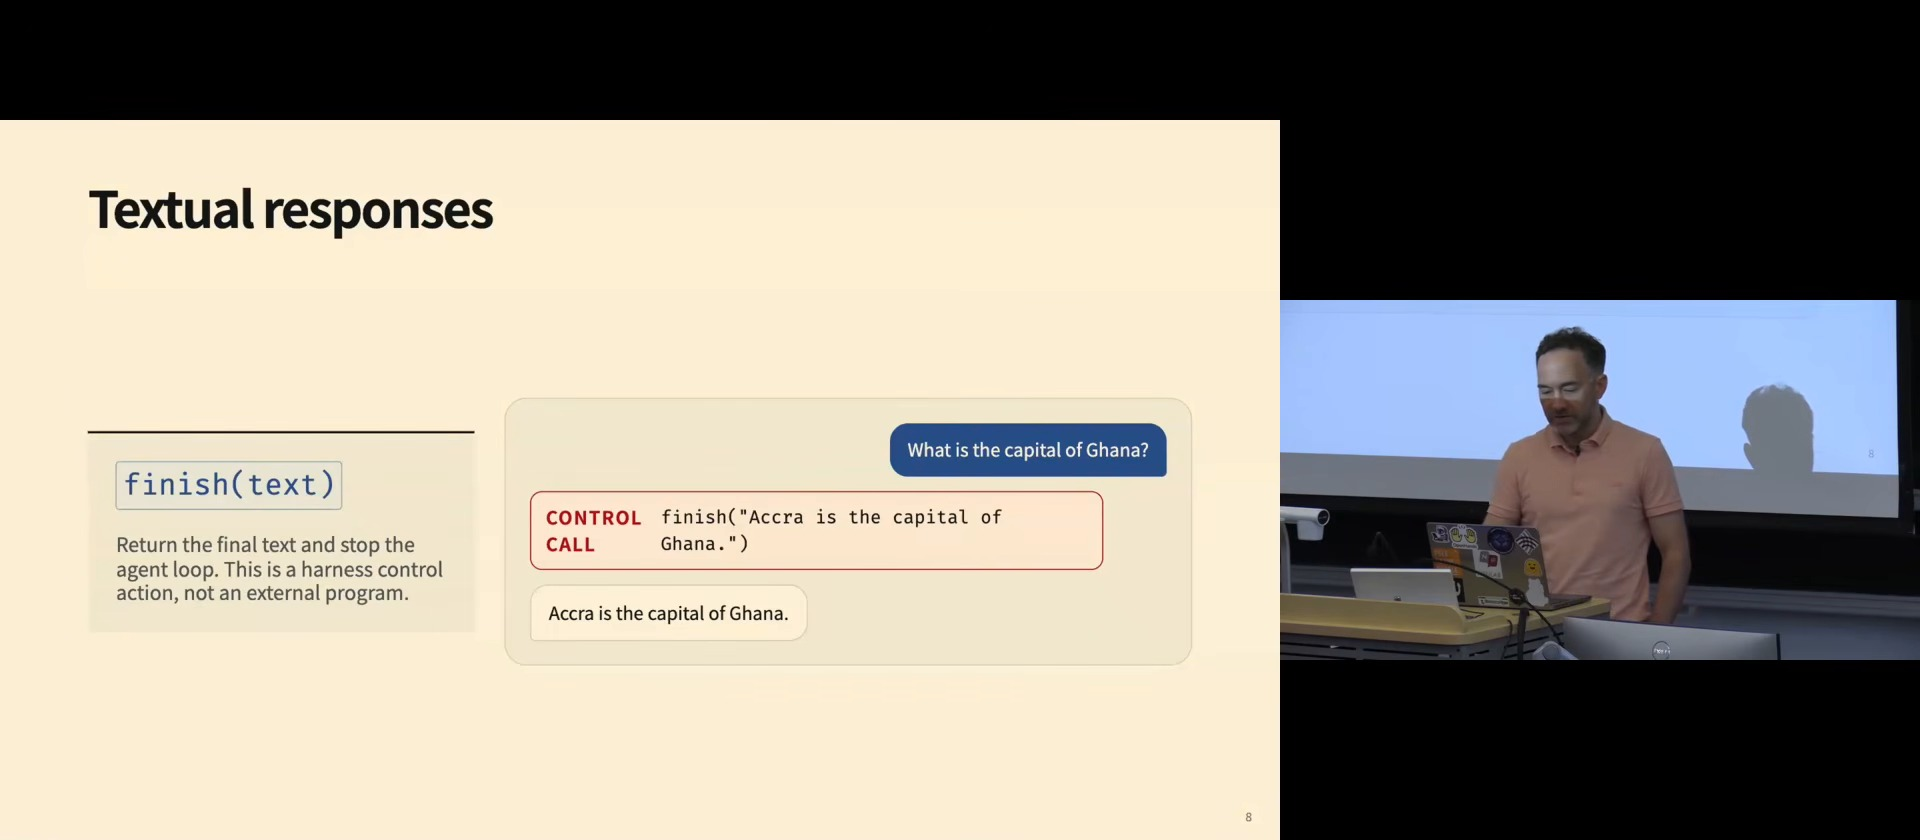
\includegraphics[width=\textwidth]{figures/fig_04_textual.jpg}
\caption{文本回复：finish(text) 让 agent loop 停止并输出最终答案，是控制动作而非外部工具\vtag}
\end{figure}
\srcnote{00:06:00--00:06:14}

\textbf{信息检索}：\texttt{search\_web(query)} 把当天网页上的内容带回上下文（例："CMU 今天宣布了三件事"）。\textbf{代码执行}：\texttt{execute\_code("sum([18,23,41,54])/4")} 在隔离环境里运行并返回 34.0。\textbf{图像生成}：\texttt{generate\_image("watercolor robot studying in a library")}——这一类与前面不同，它处理的是图像而非文本，而且模型会先把用户的简短描述\textbf{扩写}成更具体的提示词。\textbf{自定义函数}：\texttt{create\_grocery\_cart(["bananas","milk","coffee"])} 返回一个总价 \$31.42 的购物车，背后可以是 Instacart 之类的业务 API；讲者说这类接口"想加多少就加多少"。

\begin{figure}[H]
\centering
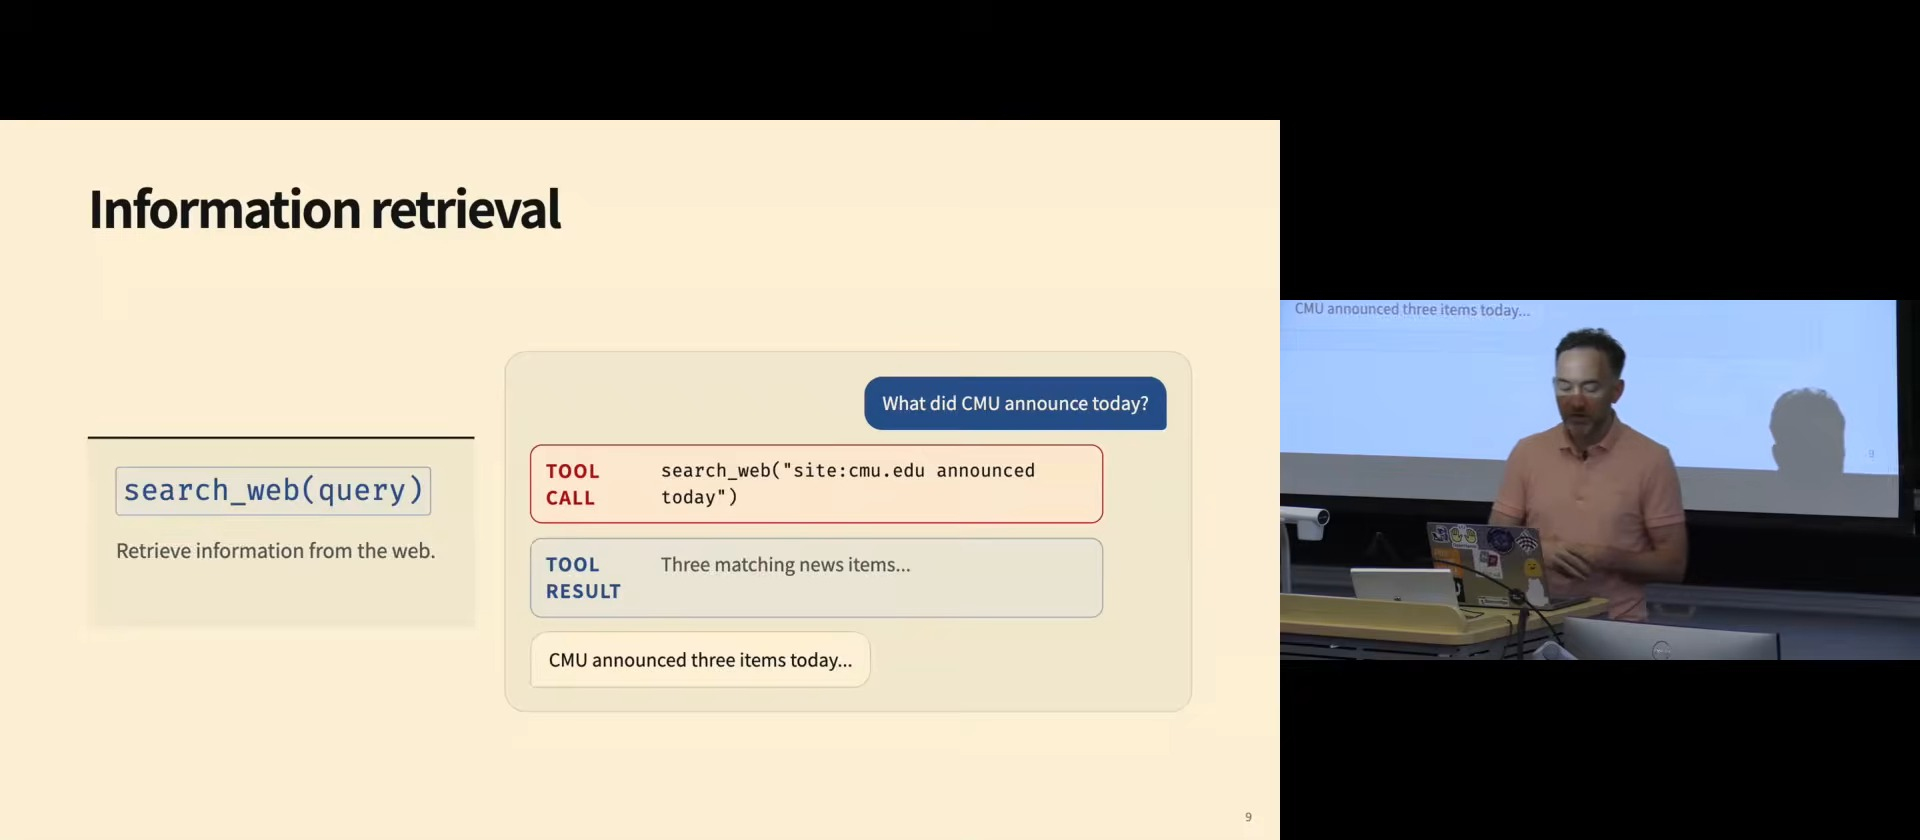
\includegraphics[width=\textwidth]{figures/fig_05_retrieval.jpg}
\caption{信息检索：search\_web 把新鲜网页内容带回上下文\vtag}
\end{figure}
\srcnote{00:07:15--00:07:29}

\begin{figure}[H]
\centering
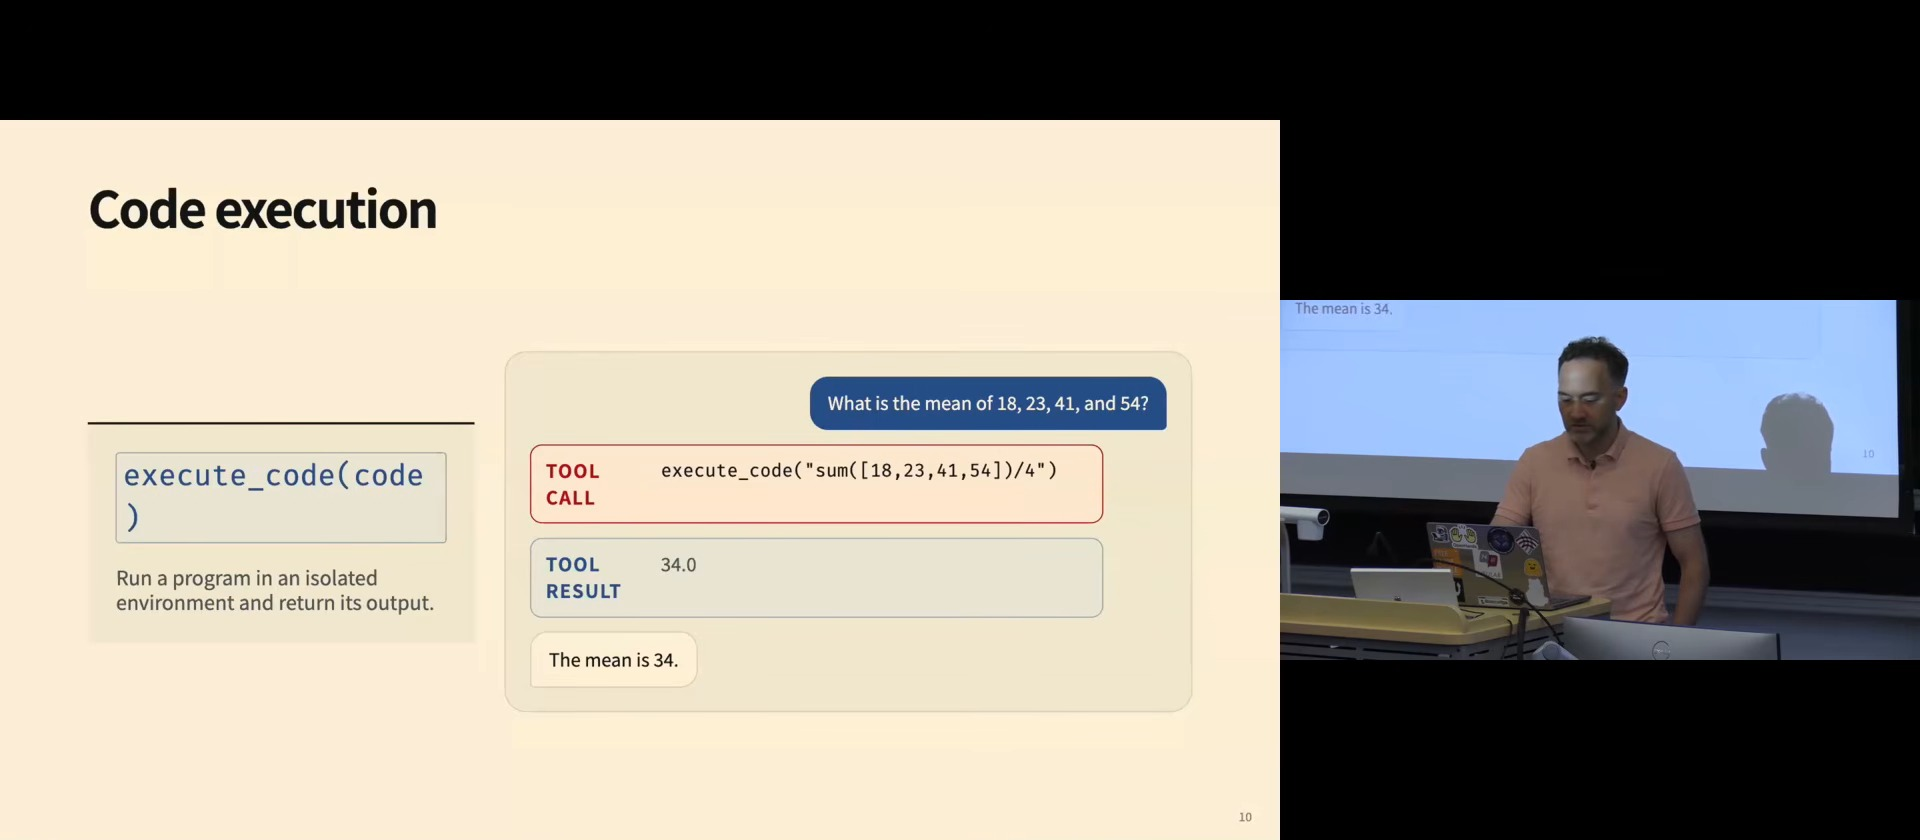
\includegraphics[width=\textwidth]{figures/fig_06_code_exec.jpg}
\caption{代码执行：在隔离环境运行表达式，返回 34.0——把推理题降级为一次调用\vtag}
\end{figure}
\srcnote{00:08:30--00:08:44}

\begin{figure}[H]
\centering
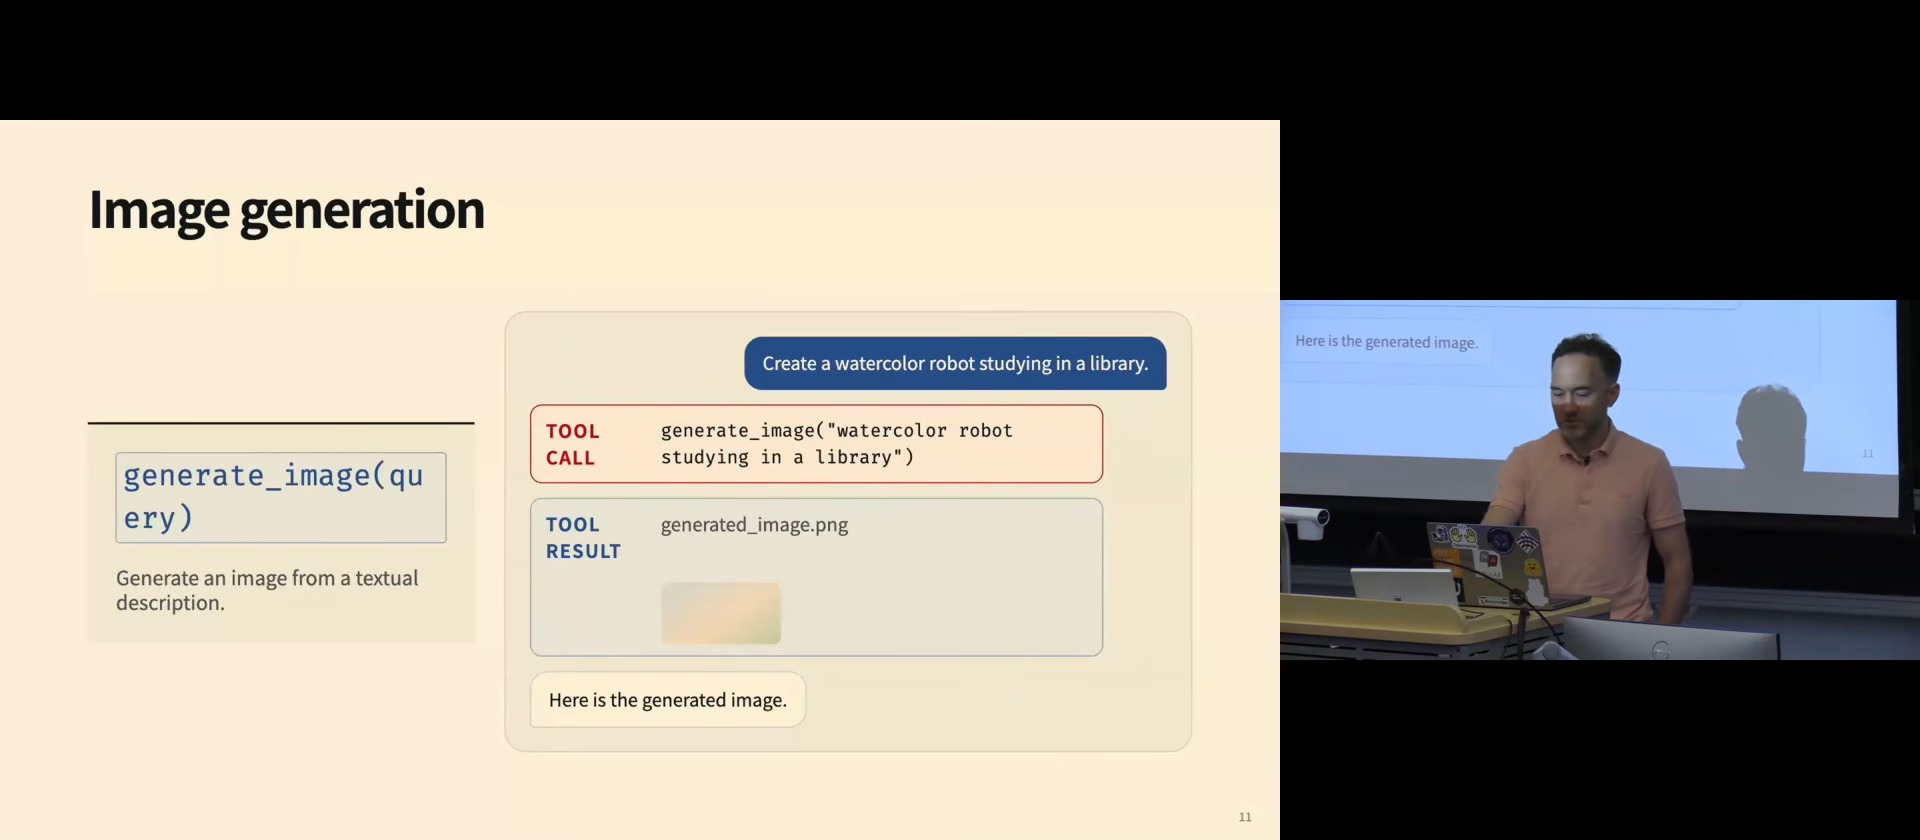
\includegraphics[width=\textwidth]{figures/fig_07_image_gen.jpg}
\caption{图像生成：模型先扩写提示词，再把更具体的 query 交给生成工具\vtag}
\end{figure}
\srcnote{00:08:45--00:08:59}

\begin{figure}[H]
\centering
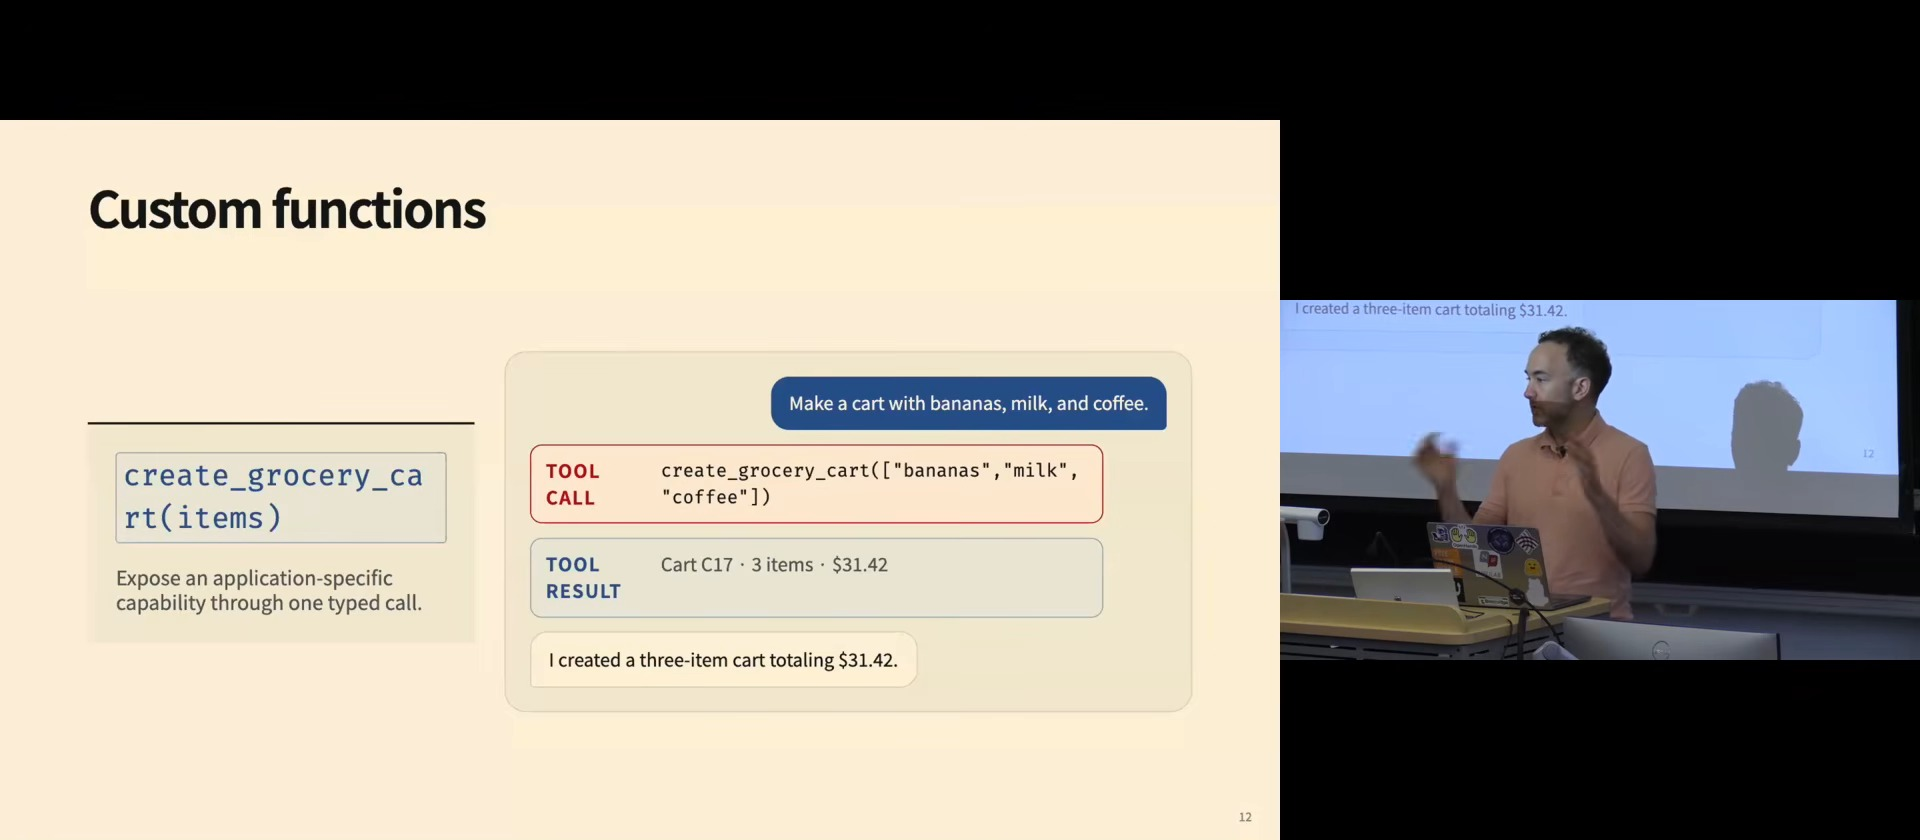
\includegraphics[width=\textwidth]{figures/fig_08_custom_fn.jpg}
\caption{自定义函数：create\_grocery\_cart 返回总价 \$31.42 的购物车，背后是业务 API\vtag}
\end{figure}
\srcnote{00:12:00--00:12:14}

\subsection{本章小结}
工具是"模型提议、系统执行"的接口；它要么补上模型做不到的能力，要么把模型能做但昂贵的事情变便宜。下一节比较两种调用范式：把 API 一个个点下去，还是让模型直接写一段程序。

\section{两种范式：逐个调用，还是写代码}

\subsection*{本节回答的问题}
"程序化工具调用"（让模型写代码来调用工具）比逐个 API 调用强在哪里，代价又是什么？

\subsection{从一次一个 API 到一段程序}

最直接的形态是给模型一份工具清单（讲者提到可能有 50 到 70 个函数），每个时间步调用其中一个；并行调用时一次发出多个。另一种形态是把\textbf{代码本身当作工具}：模型写出一段程序，程序里调用各种接口。

代码之所以特殊，是因为它是一个\textbf{元工具}：语言内建函数是工具，外部库（比如 pandas）等于一次性打开几百个工具，自定义的工具函数也能被同一段程序组合起来。讲者用"200 个面包卖出若干还剩多少"这类题目说明：代码里的赋值、减法、循环，本质都是在调用"工具"，只是粒度更细。

\begin{importantbox}{代码是"工具之上的工具"}
逐个 API 调用是"一步一个动作"；代码化调用是"一次写出动作的组合方案"。它把若干次串行决策压缩成一次生成，因此既更表达力强，也更省往返——这正是下面那段实测要说明的事。
\end{importantbox}

\subsection{程序化组合：一次生成 vs 十次往返}

幻灯片给了一个只有五个 API 的任务：判断在哪个国家买某型号手机最划算，候选是美国、日本、德国、印度；可用 API 只有 \texttt{lookup\_rates}、\texttt{lookup\_phone\_price}、\texttt{convert}、\texttt{estimate\_final\_price}。如果一次调用一个 API，agent 会陷入"查汇率 → 查价格 → 转换 → 再查汇率 ……"的长循环；如果允许写代码，它可以一次写出遍历四个国家、逐个估算并比较的完整程序。

\begin{equation}
A(x) \;=\; f_n\bigl(\cdots f_2\bigl(f_1(x)\bigr)\cdots\bigr)
\end{equation}
式中 $x$ 为输入，$f_i$ 为可调用的工具函数，$A(x)$ 为最终结果。逐个调用时，这棵调用树要分 $n$ 次生成才展开完；代码化调用把整棵树放进\textbf{一次}生成里，之后只在环境里执行——这解释了为什么后者的交互轮数会显著下降。

\begin{figure}[H]
\centering
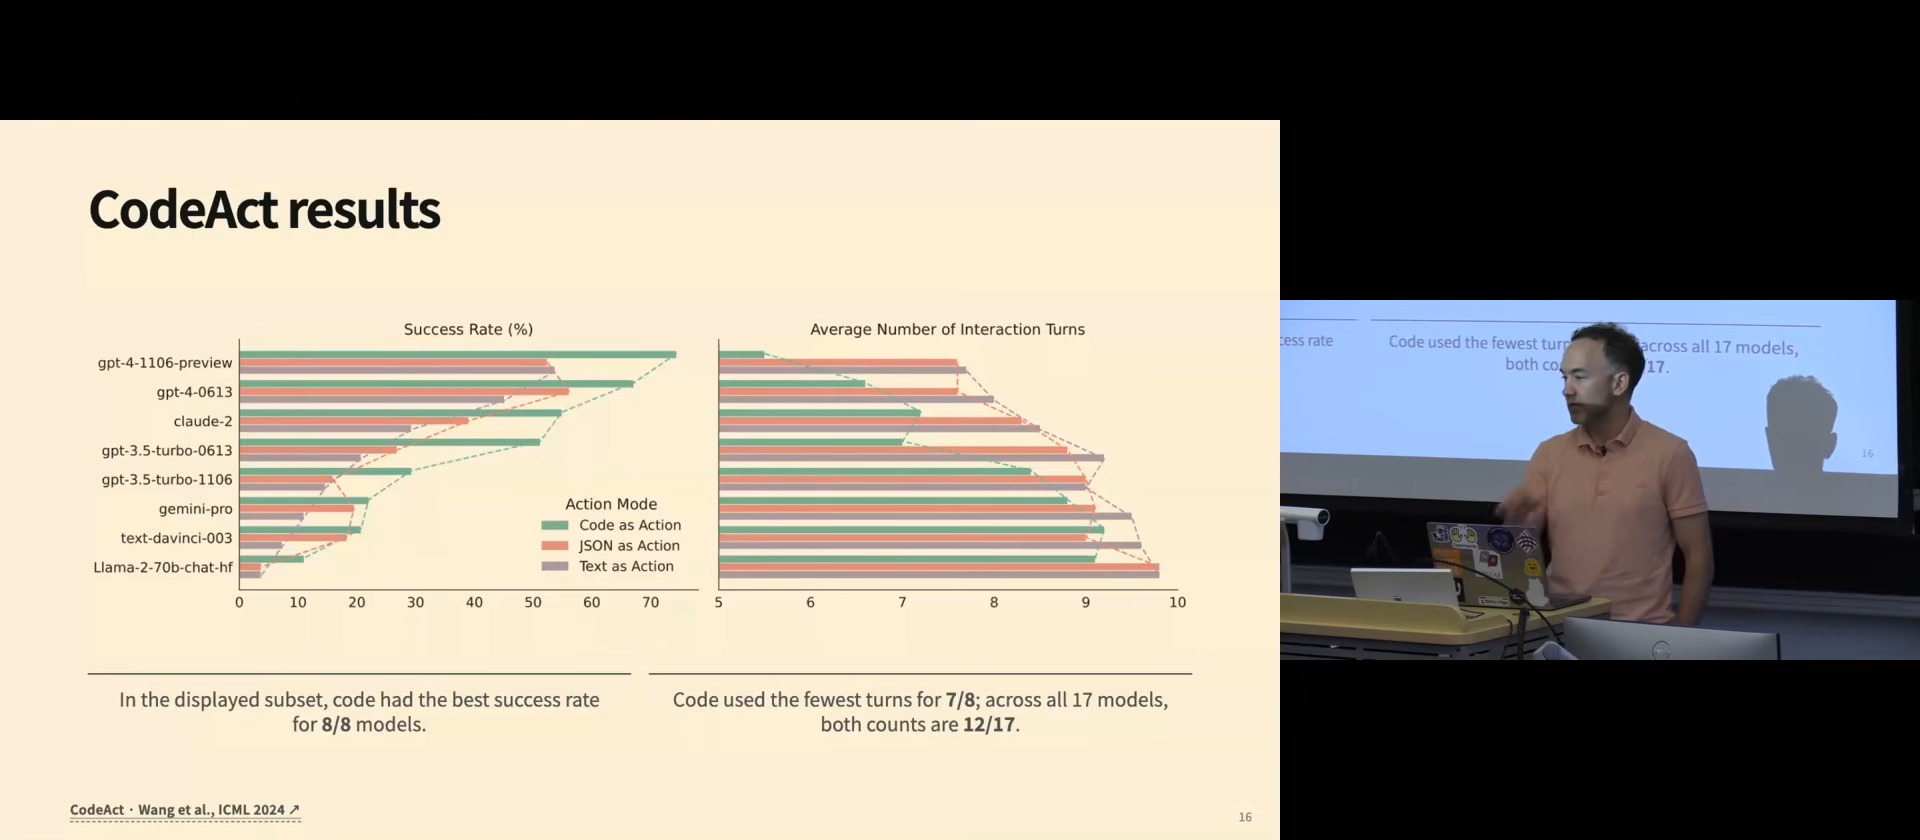
\includegraphics[width=\textwidth]{figures/fig_09_codeact_result.jpg}
\caption{CodeAct 结果：横轴成功率、纵轴平均交互轮数；代码方案在 17 个模型上都用最少轮数\vtag}
\end{figure}
\srcnote{00:14:00--00:14:14}

讲者引用的是 CodeAct 一类的实证工作：把工具调用写成代码，\textbf{成功率上升、平均交互轮数下降}，而且这一优势不限于"看起来就该写代码"的任务——即使是传统上被当作普通工具调用的任务，写成代码也更划算。

\subsection{代价：高功率意味着高风险}

代码强，但不是万金油。幻灯片把代价列成两列对照：左侧是\textbf{表达力}（循环、变量、库；非常适合多步数据处理与组合），右侧是\textbf{更难约束}——动作空间宽（文件、网络、进程都可能被触碰）、影响面大，因此需要沙箱、资源限制与校验。课堂上学生补了两个具体风险：\textbf{死循环}（模型可能写出永不结束的循环，系统必须有兜底）与\textbf{依赖投毒}（agent 拉进一个被攻陷的第三方库，整个系统随之失守——这是当前 agent 网络安全的主要风险之一）。

\begin{figure}[H]
\centering
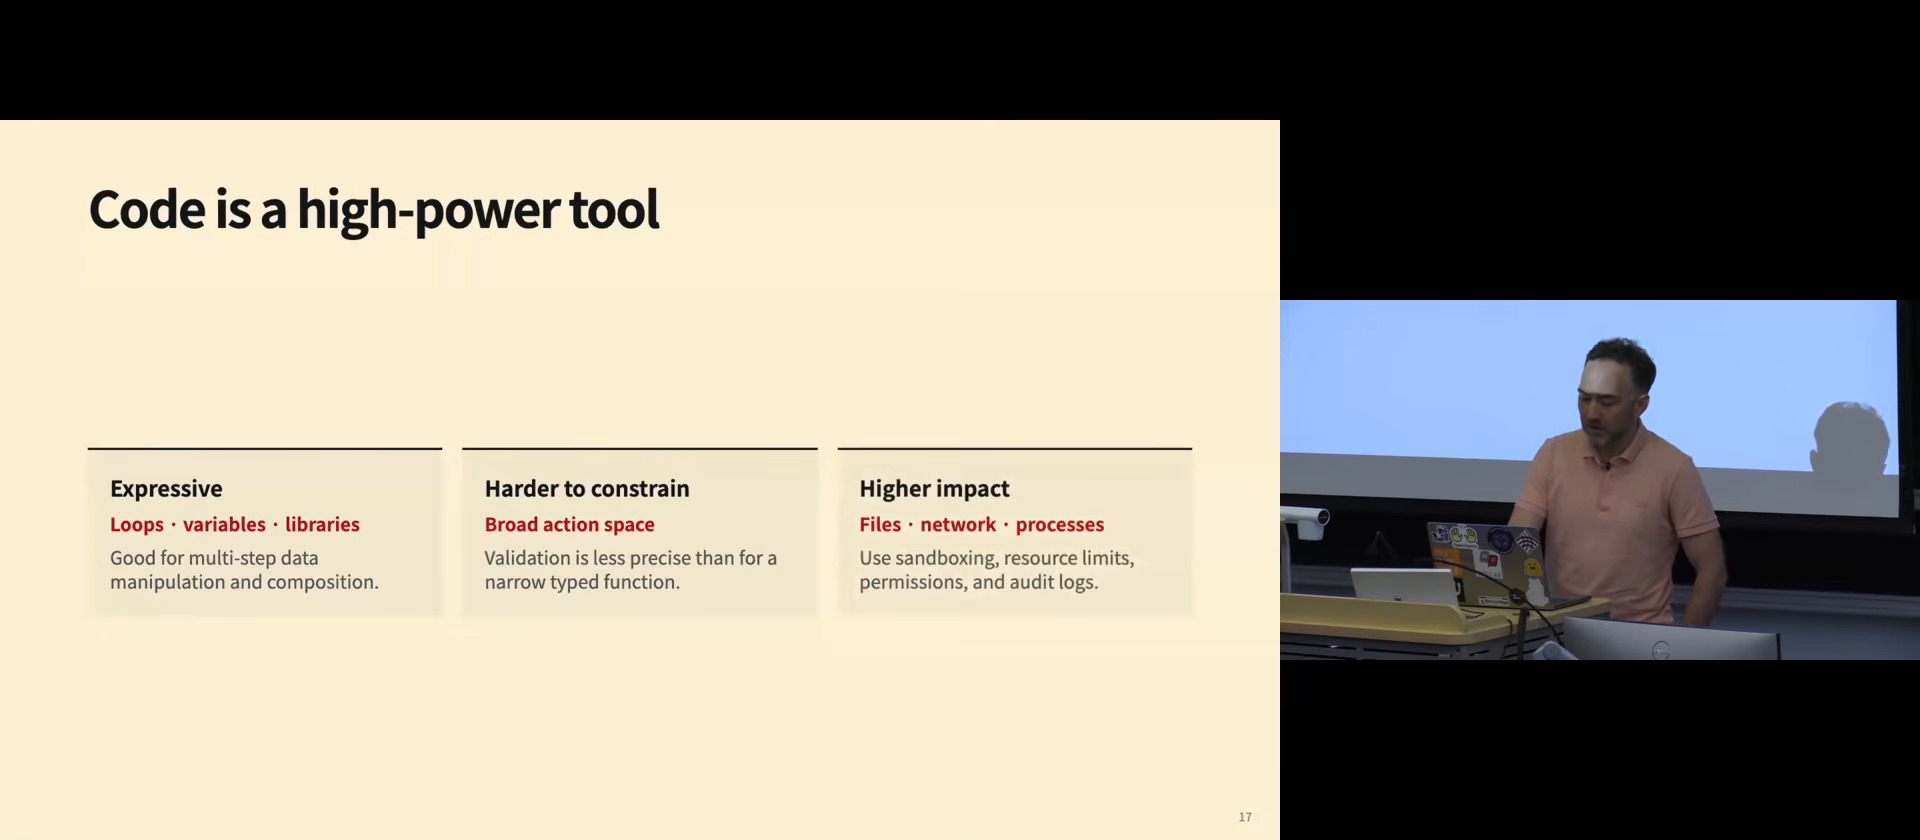
\includegraphics[width=\textwidth]{figures/fig_10_code_power.jpg}
\caption{代码是高功率工具：表达力强、适合多步组合，但动作空间宽、更难约束、影响面大\vtag}
\end{figure}
\srcnote{00:15:30--00:15:44}

\begin{warningbox}{一旦允许写代码，就必须先回答三个问题}
\textbf{（1）兜底}：无限循环、超长运行、内存暴涨由谁终止？\textbf{（2）隔离}：文件、网络、进程的权限边界在哪里？\textbf{（3）来源}：允许安装哪些依赖，如何防止供应链投毒？这三个问题没有答案时，程序化工具调用带来的收益会被风险吃掉——课程在后面专门讲安全时还会回到这里。
\end{warningbox}

\subsection{本章小结}
两种范式并不互斥：窄任务用结构化调用更稳，多步组合用代码更省。无论哪一种，调用最终都要变成模型输出的一段 token，再由系统执行——这正是下一节的主题。

\section{机制：工具调用如何变成动作}

\subsection*{本节回答的问题}
一次工具调用在模型侧长什么样？不同模型为什么不能通用解析？系统侧又如何把调用派发出去、把结果收回来？

\subsection{工具调用就是 token 序列}

幻灯片把两种续写并列：文本续写是 \texttt{The weather is sunny.}，工具续写是一段 \texttt{<tool\_call>} 片段（例如 \texttt{get\_weather(...)}）。两者没有本质区别——都是模型预测出来的 token 序列，区别只在于系统如何解释它。

\begin{equation}
y_t \;=\; c_t \;\oplus\; m_t \;\oplus\; a_t
\end{equation}
式中 $y_t$ 为第 $t$ 步的完整输出，$c_t$ 为思考 token（内部推理，通常不展示），$m_t$ 为给用户看的自然语言消息，$a_t$ 为工具调用片段，$\oplus$ 表示按顺序拼接。讲者指出：ReAct 那种"想一步、说一句、调一次"的循环，今天往往就是\textbf{一次生成}里的三段内容，而不是框架代码拼出来的多段。

\begin{figure}[H]
\centering
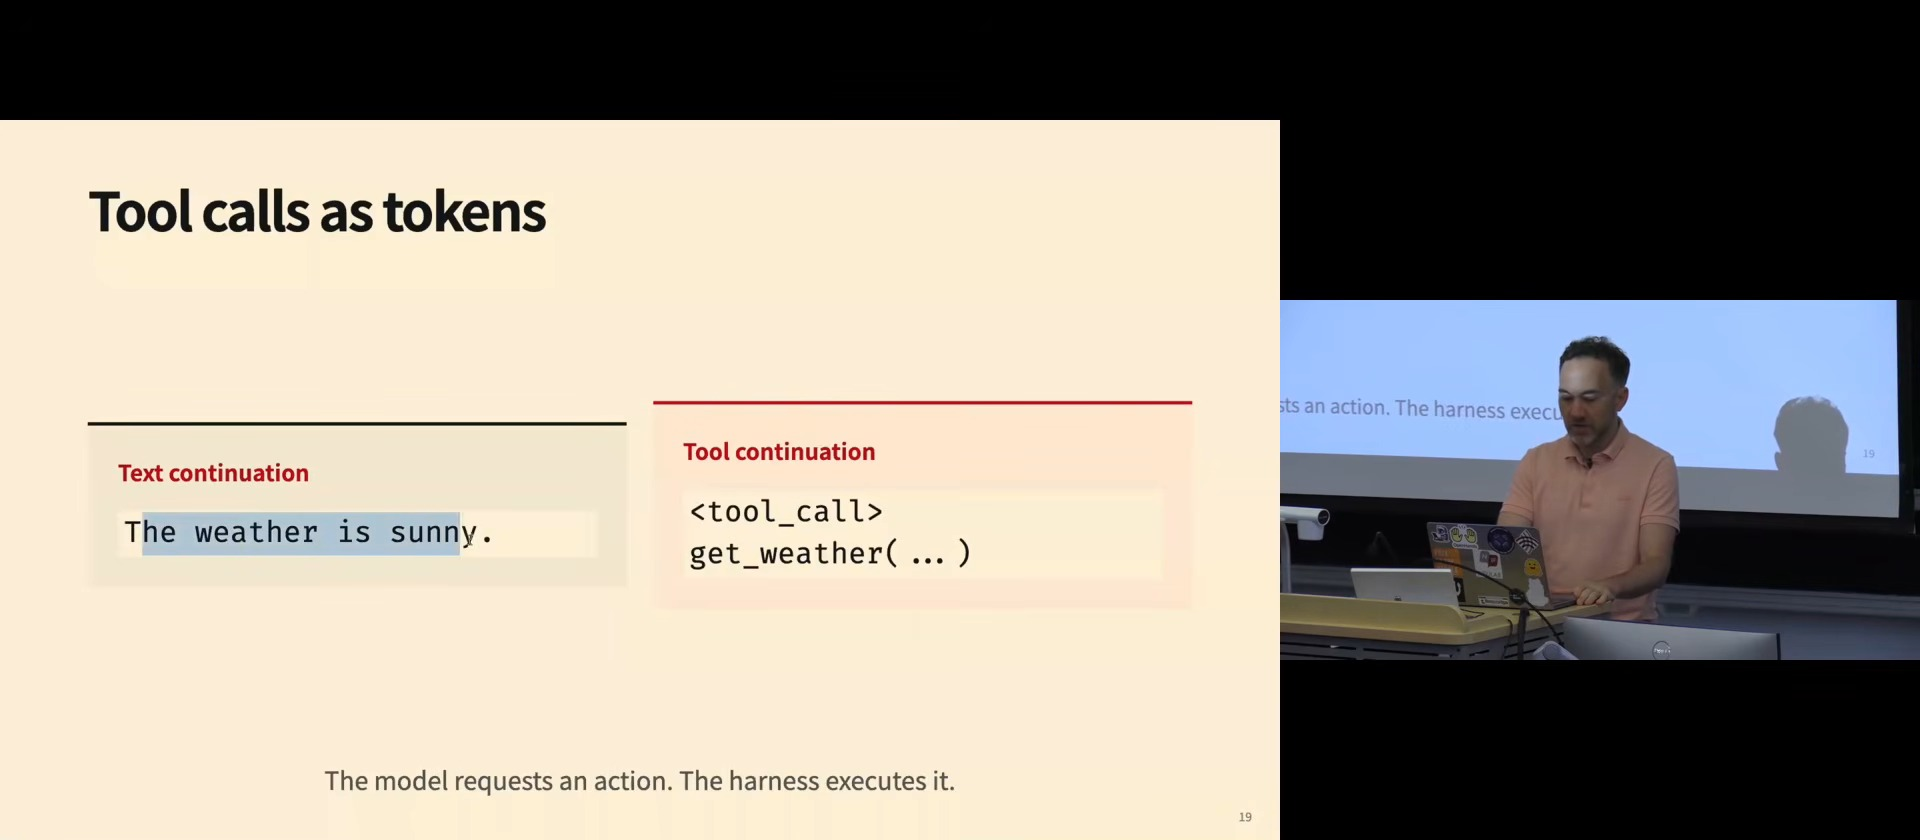
\includegraphics[width=\textwidth]{figures/fig_11_calls_as_tokens.jpg}
\caption{工具调用即 token：文本续写与工具续写同源，后者由 harness 解释并执行\vtag}
\end{figure}
\srcnote{00:16:30--00:16:44}

课堂上有人问：这些特殊 token 是否必须在预训练时就进词表？讲者的回答很实用：预训练阶段通常没有，它们多在 \textbf{mid-training}（用指令、轨迹与工具调用数据训练）阶段被引入；而微调者要做的，是沿用模型已经被训练过的格式。

\subsection{聊天模板与工具定义}

一次 API 请求里的消息（system / user / assistant）在送给模型前，会被聊天模板序列化成带控制 token 的一条序列；工具定义则给这份请求加上了结构：\texttt{type}、\texttt{function}、\texttt{name}、\texttt{parameters} 等字段。提示里出现 \texttt{<tools>} 定义块，模型吐出 \texttt{<tool\_call>} JSON，API 响应再给这次调用补一个 call ID。

\begin{figure}[H]
\centering
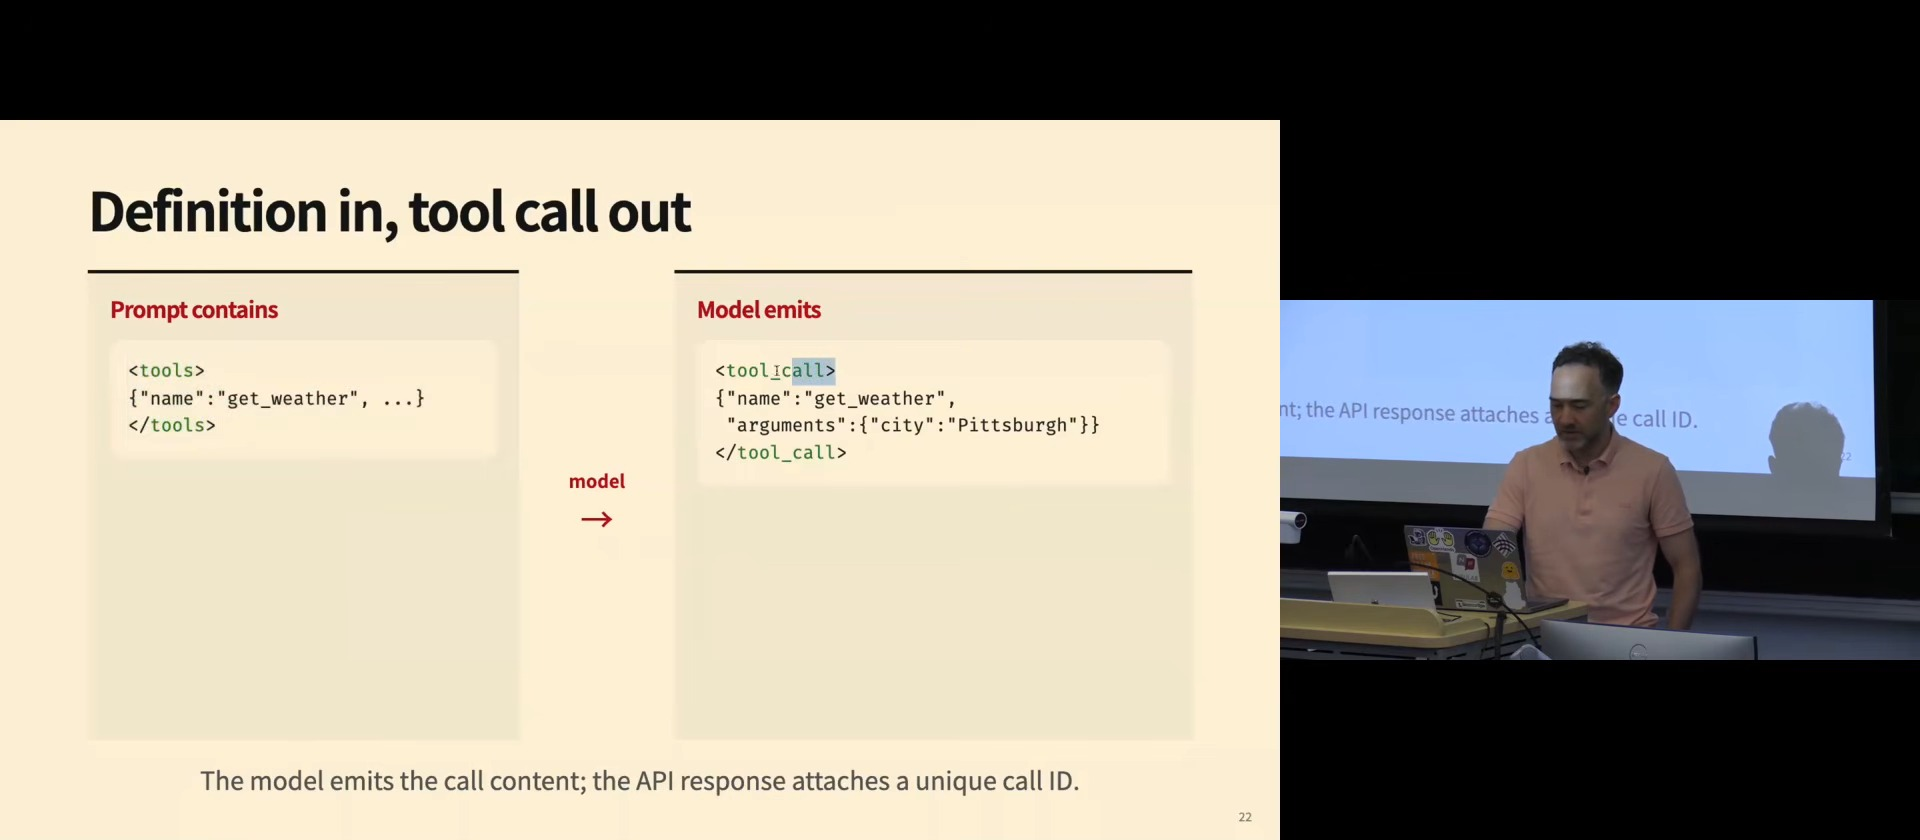
\includegraphics[width=\textwidth]{figures/fig_12_tool_structure.jpg}
\caption{定义进、调用出：提示里是 <tools> 定义，模型输出 <tool\_call> JSON，响应回填 call ID\vtag}
\end{figure}
\srcnote{00:20:45--00:20:59}

\begin{importantbox}{一次工具调用的完整链路}
\textbf{（1）}工具定义进入请求；\textbf{（2）}模板把定义与历史渲染成一条模型输入序列；\textbf{（3）}模型生成调用片段；\textbf{（4）}系统解析、校验并执行；\textbf{（5）}结果与 call ID 配对回填为一条 tool 消息；\textbf{（6）}模型带着新观测继续生成。任何一个环节的格式假设出错，整条链都会断。
\end{importantbox}

\subsection{协议各不相同：一个真实的工程陷阱}

同一个 \texttt{get\_weather} 调用，三家模型用了三种表示：Qwen 3.8 用控制 token 加 call ID，Mistral Small 4 用函数与参数标签，DeepSeek V3.2 用 DSML 调用块。讲者强调这不是小道消息，而是必须知道的工程事实：\textbf{为 DeepSeek 写的解析代码不会自动支持 Qwen}，反之亦然。

\begin{figure}[H]
\centering
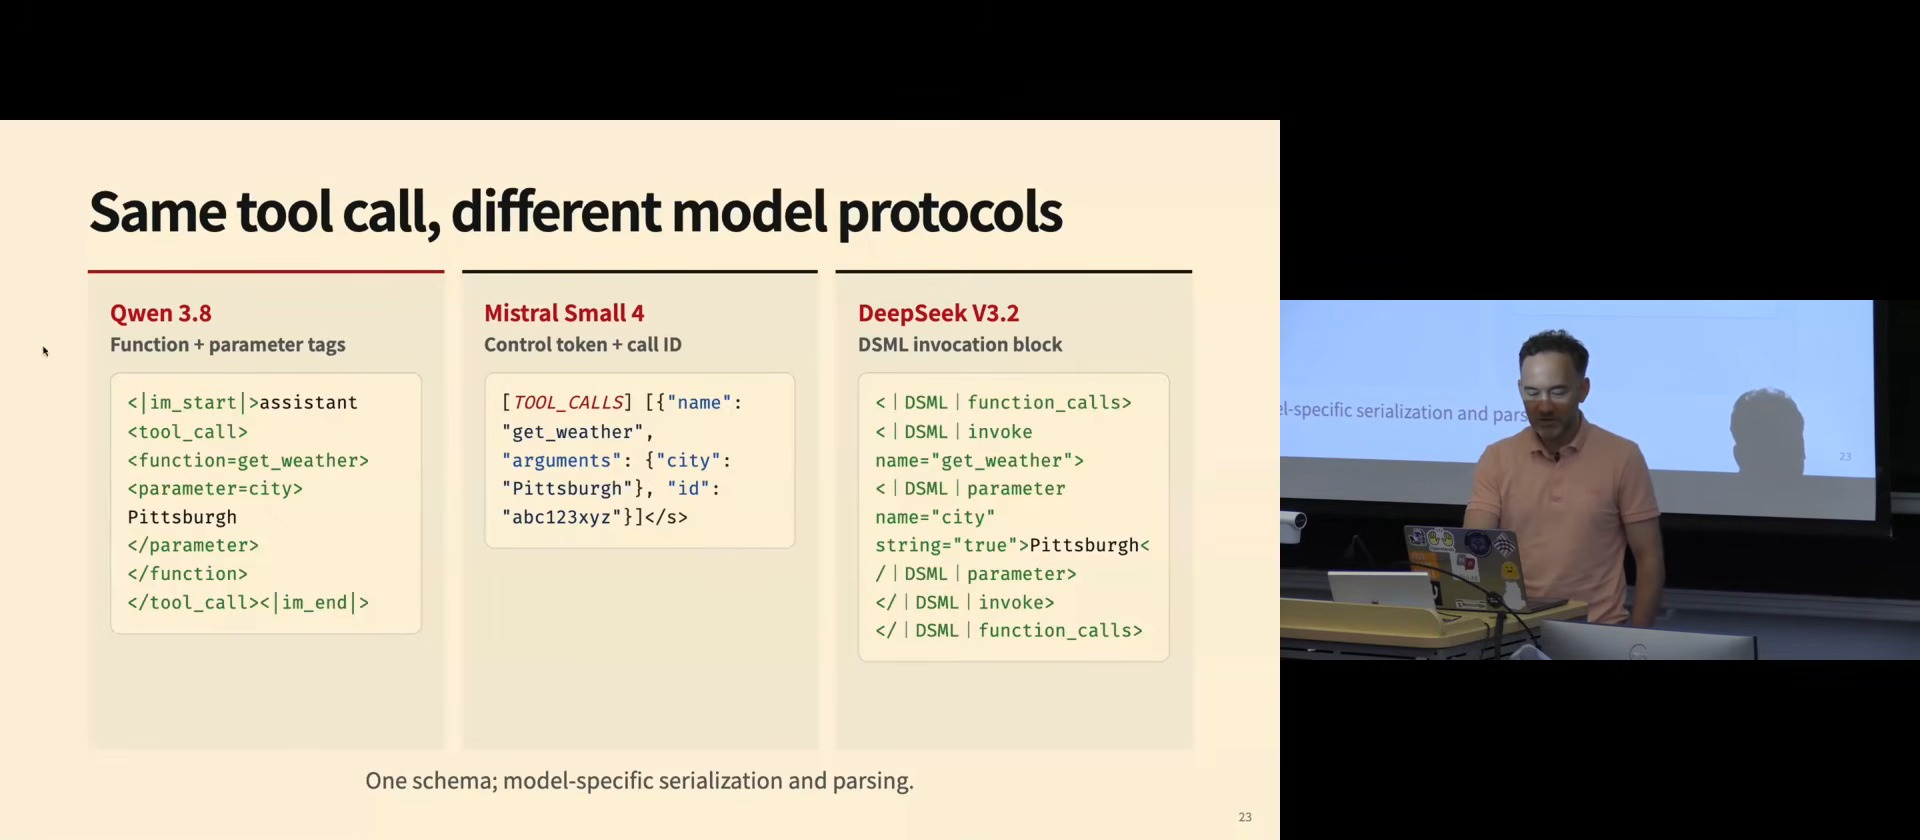
\includegraphics[width=\textwidth]{figures/fig_13_protocols.jpg}
\caption{同一个工具调用、三种协议：Qwen 3.8（控制 token + call ID）、Mistral Small 4（函数与参数标签）、DeepSeek V3.2（DSML 块）\vtag}
\end{figure}
\srcnote{00:21:15--00:21:29}

\begin{knowledgebox}{别自己发明协议}
Hugging Face 的 \texttt{apply\_chat\_template} 已经把主流模型的模板实现好了；讲者的建议是\textbf{从已有模型微调时，100\% 沿用它的工具调用格式}，不要试图教会它一套新写法，也不要自己手写解析器去猜格式。格式差异带来的 bug 通常出现在最不起眼的地方：把 A 模型的输出喂给 B 模型的解析器。
\end{knowledgebox}

\subsection{系统侧：注册、校验、执行、配对}

系统侧的第一步是\textbf{初始化时注册}：把工具名映射到定义与执行器（幻灯片用 \texttt{tools\_map[name]}、\texttt{resolve\_tool(spec,state)} 表示）。运行时按名字查表、用参数执行，并把结果返回。

\begin{figure}[H]
\centering
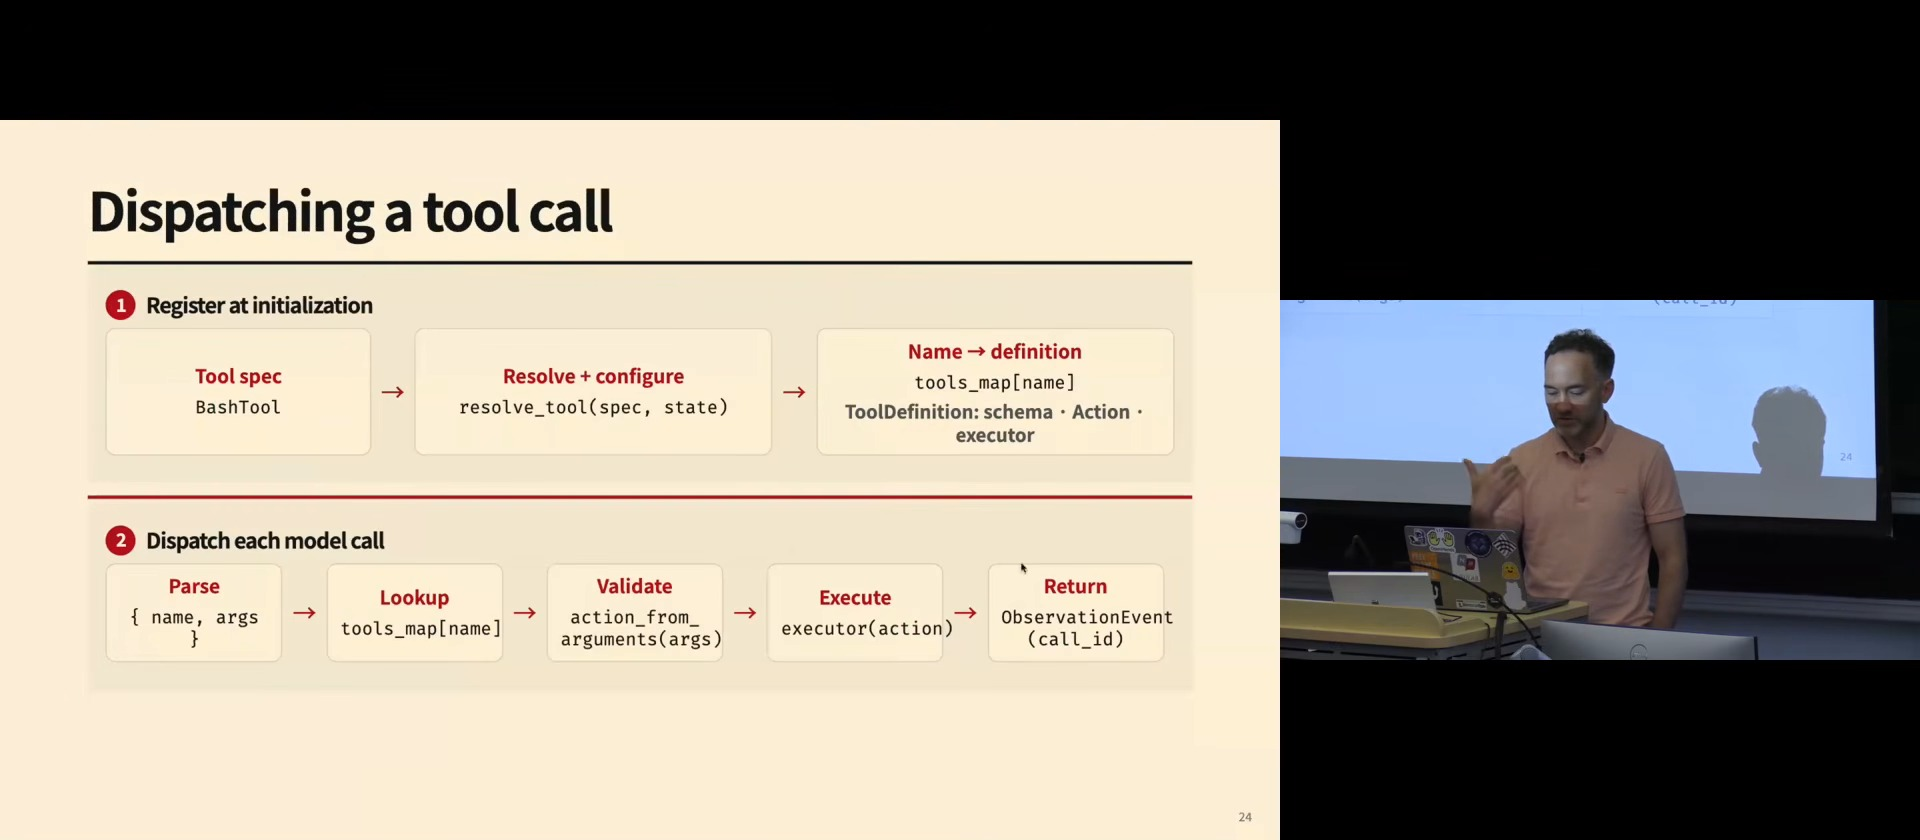
\includegraphics[width=\textwidth]{figures/fig_14_dispatch.jpg}
\caption{分发一次调用：初始化注册 name→definition，运行时解析并派发到具体 Tool（如 BashTool）\vtag}
\end{figure}
\srcnote{00:23:45--00:23:59}

失败分两类：\textbf{校验失败}（模型给了不存在的字段或错误类型）与\textbf{执行失败}（格式合法但语义非法，例如一段语法正确却会抛异常的 Python）。两类失败都要作为观测送回模型，让它有机会修正——这也是 agent 比单次调用更稳的原因之一。

结果用 \textbf{call ID} 与调用配对：assistant 消息里的 \texttt{tool\_calls} 带 \texttt{id}，随后 role 为 \texttt{tool} 的消息用 \texttt{tool\_call\_id} 指回同一个 id。在并行调用时，这层配对是唯一能分清"哪个结果属于哪个调用"的线索。

\begin{figure}[H]
\centering
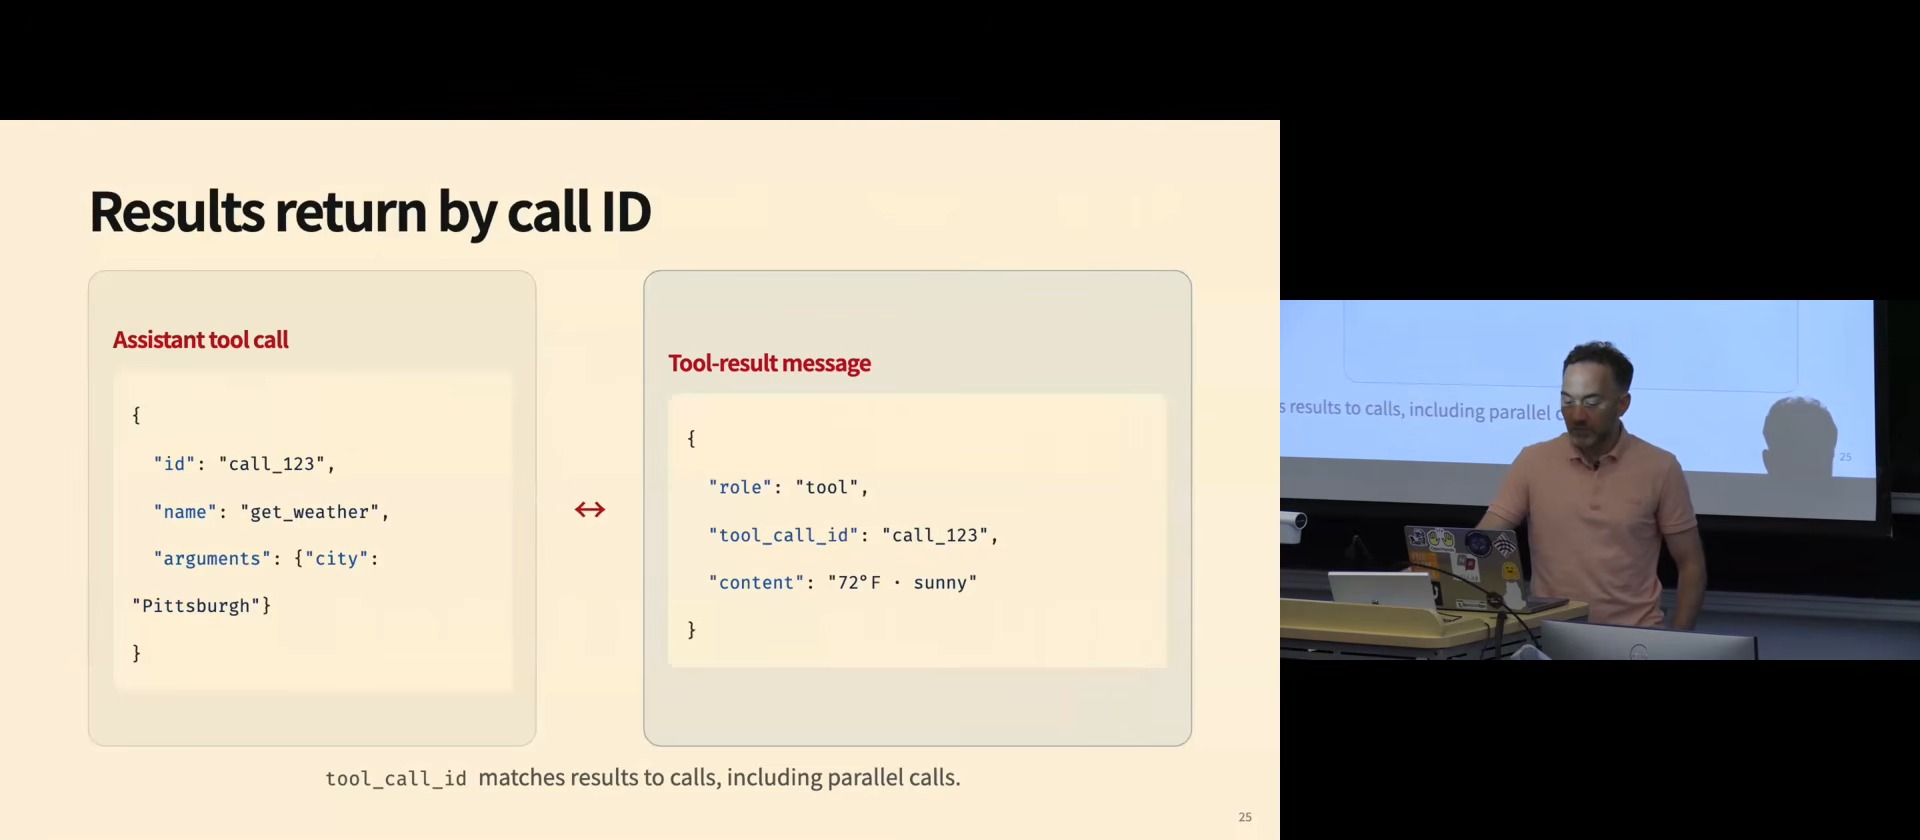
\includegraphics[width=\textwidth]{figures/fig_15_call_id.jpg}
\caption{结果按 call ID 回填：assistant 的 tool\_calls 与 role=tool 的 tool\_call\_id 一一对应\vtag}
\end{figure}
\srcnote{00:25:15--00:25:29}

\begin{warningbox}{history 的合法性是硬约束}
讲者特别提醒：某些模型（例如 Anthropic 系列）会直接拒绝"有调用、无结果"的历史。实践中最容易踩的场景是——agent 发出工具调用后程序崩溃，恢复时缺了那条结果消息，于是整个会话再也无法继续。恢复逻辑必须保证\textbf{调用与结果成对出现}，或者显式地把残缺历史补齐/丢弃。
\end{warningbox}

\subsection{本章小结}
工具调用的物理形态是一段 token，工程形态是一条包含"定义—渲染—生成—校验—执行—配对"的流水线，而各家协议并不统一。既然如此，系统就不该指望模型每次都写对格式；下一节讲怎么让格式在解码阶段就不可能出错。

\section{约束解码：让调用不可能写错}

\subsection*{本节回答的问题}
为什么模型会写出畸形调用？约束解码用什么机制保证格式合法，它的边界又在哪里？

\subsection{畸形调用与四类约束}

语言模型不保证输出合法结构——幻灯片给了一个最典型的例子：一段 JSON 少了最后的右花括号，解析器直接抛异常，整个 agent 卡住。讲者说见过太多人试图在事后"补括号"，他的态度很明确：不要靠字符串修补，要在生成阶段就约束住。

\begin{figure}[H]
\centering
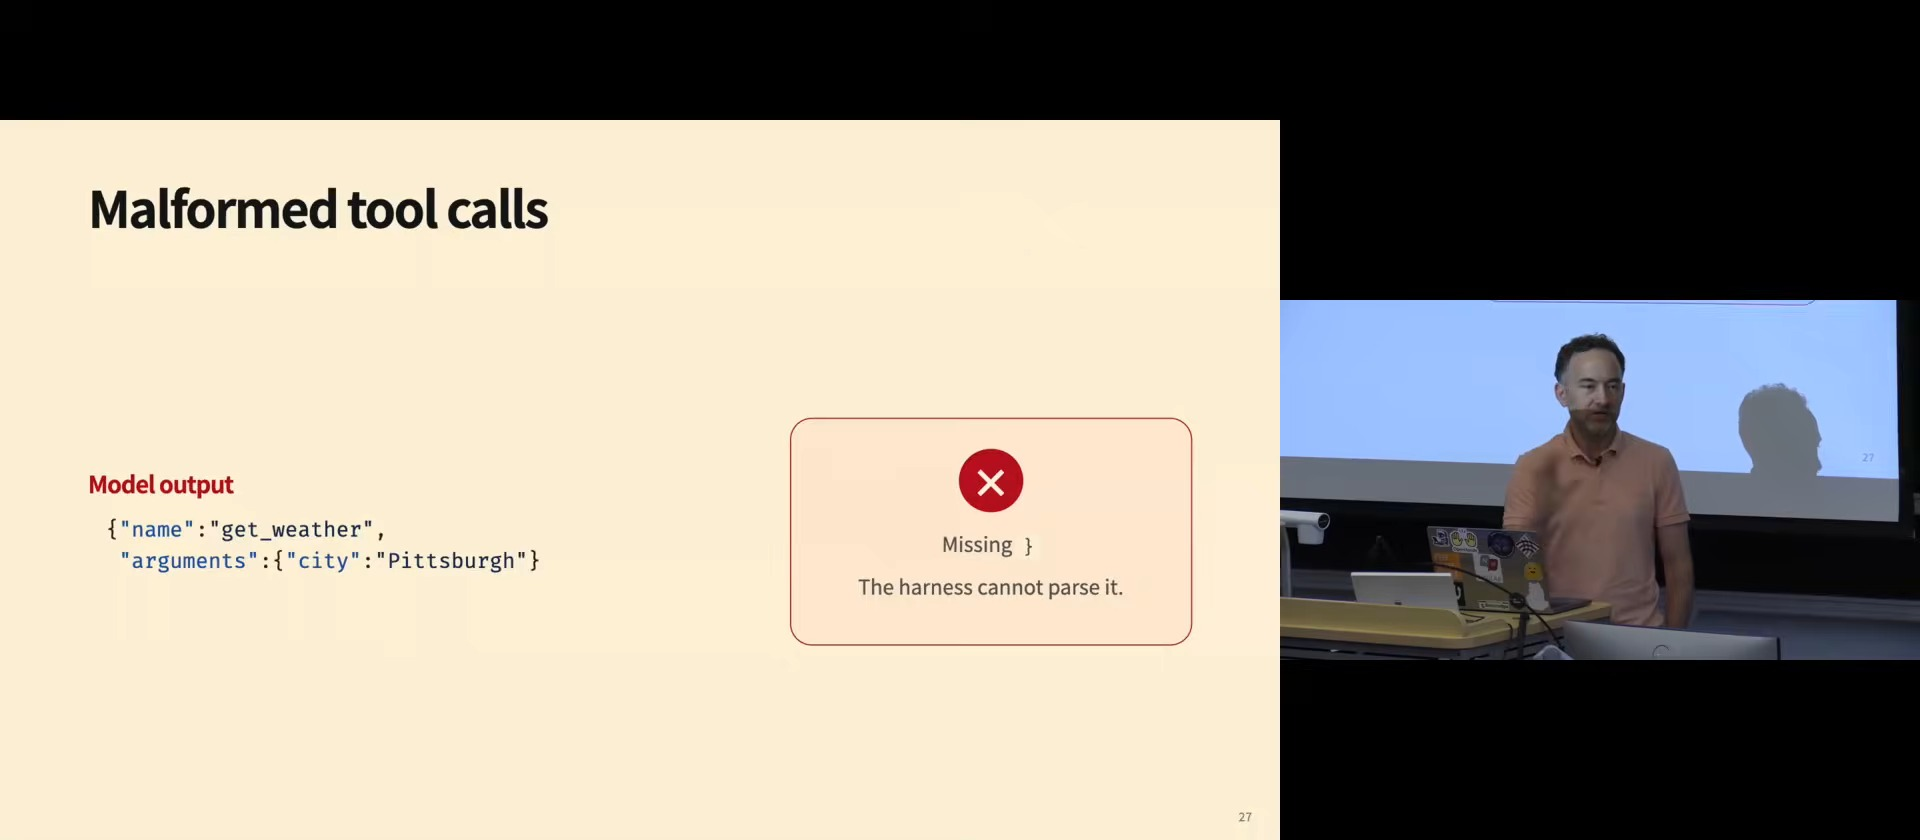
\includegraphics[width=\textwidth]{figures/fig_16_malformed.jpg}
\caption{畸形调用：JSON 缺一个右括号，harness 无法解析——事后补括号不是工程做法\vtag}
\end{figure}
\srcnote{00:27:30--00:27:44}

调用需要同时满足四层约束：

\begin{center}
\small
\begin{tabular}{lll}
\toprule
层次 & 要求 & 例子 \\
\midrule
Syntax（语法） & 是合法的 JSON & 括号、逗号完整 \\
Shape（形状） & 必填字段齐全 & \texttt{city} 必须出现 \\
Types（类型） & 字段类型正确 & \texttt{city} 是字符串 \\
Values（取值） & 落在允许的取值集合内 & \texttt{units} 只能是 C 或 F \\
\bottomrule
\end{tabular}
\end{center}

\begin{figure}[H]
\centering
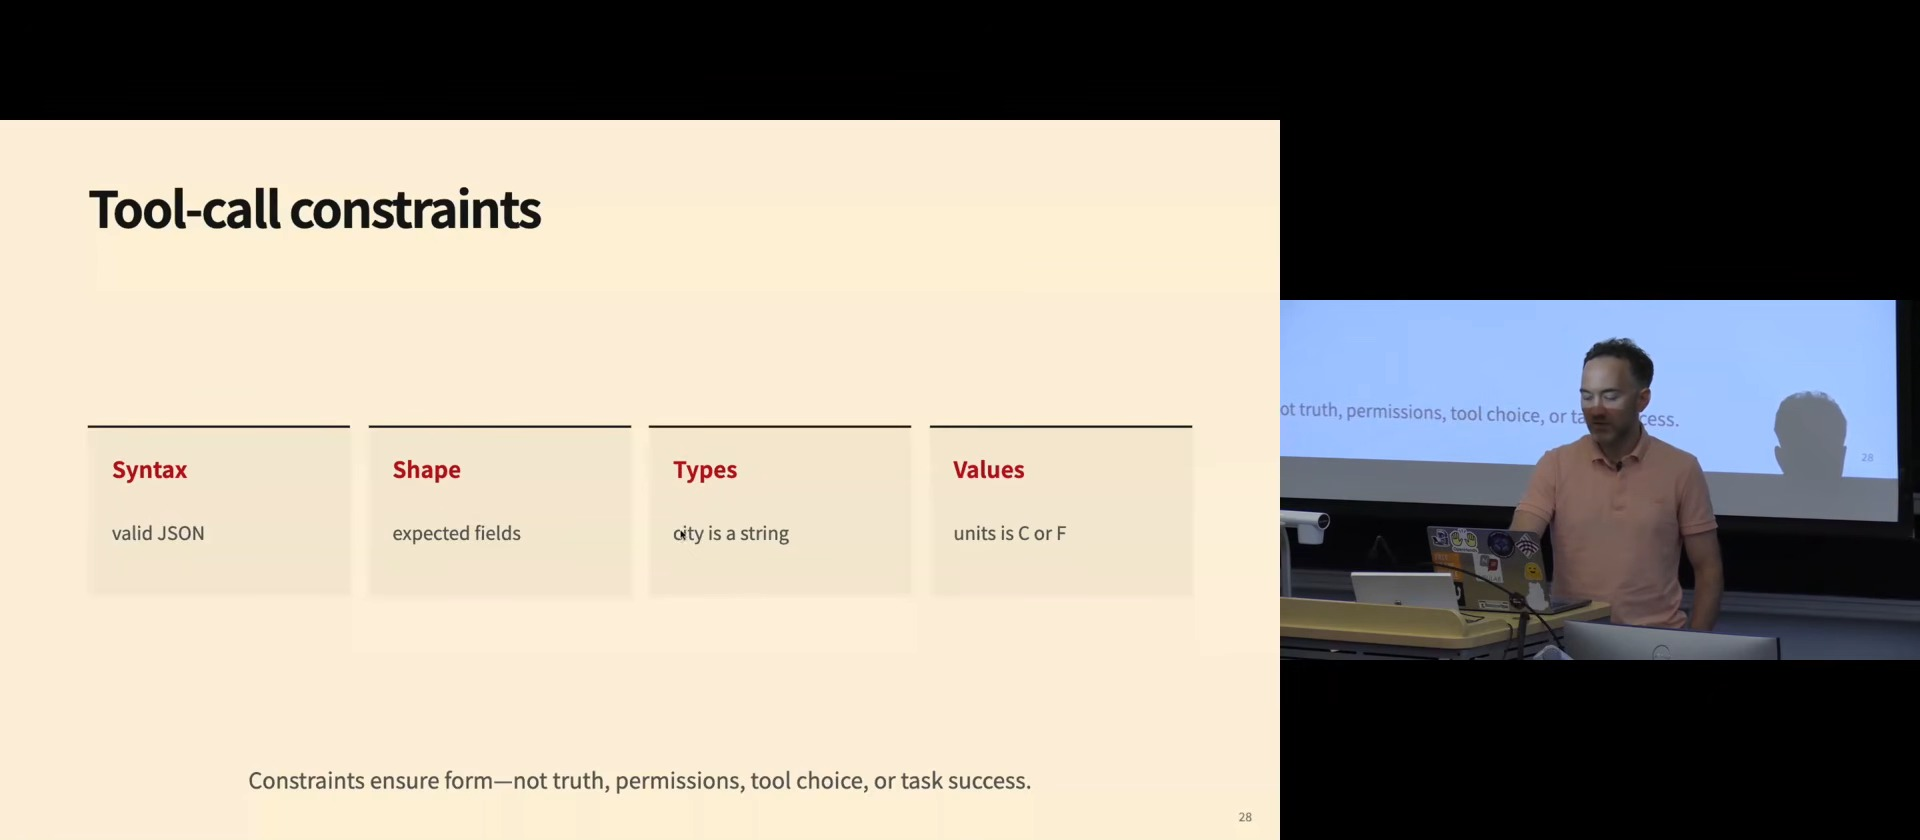
\includegraphics[width=\textwidth]{figures/fig_17_constraints.jpg}
\caption{四类约束：syntax / shape / types / values；它们只保证形式，不保证真值、权限与工具选择\vtag}
\end{figure}
\srcnote{00:28:15--00:28:29}

这张图右下角那句话值得单独记住：\textbf{约束保证的是形式（form），不是真值（truth）、权限（permissions）或工具选择（tool choice）}。一个完全符合 schema 的调用，仍然可能是一个错误的决定——约束解码解决的是"能不能被解析"，不是"该不该这么做"。

\subsection{JSON Schema 与语法树}

JSON Schema 是"描述 JSON 数据的词汇表"：类型、必填字段、枚举取值范围都可以写进去，而且机器可读。幻灯片给的例子声明对象有 \texttt{city}（字符串）与 \texttt{units}（枚举 C/F），\texttt{city} 必填，额外属性不允许。

\begin{figure}[H]
\centering
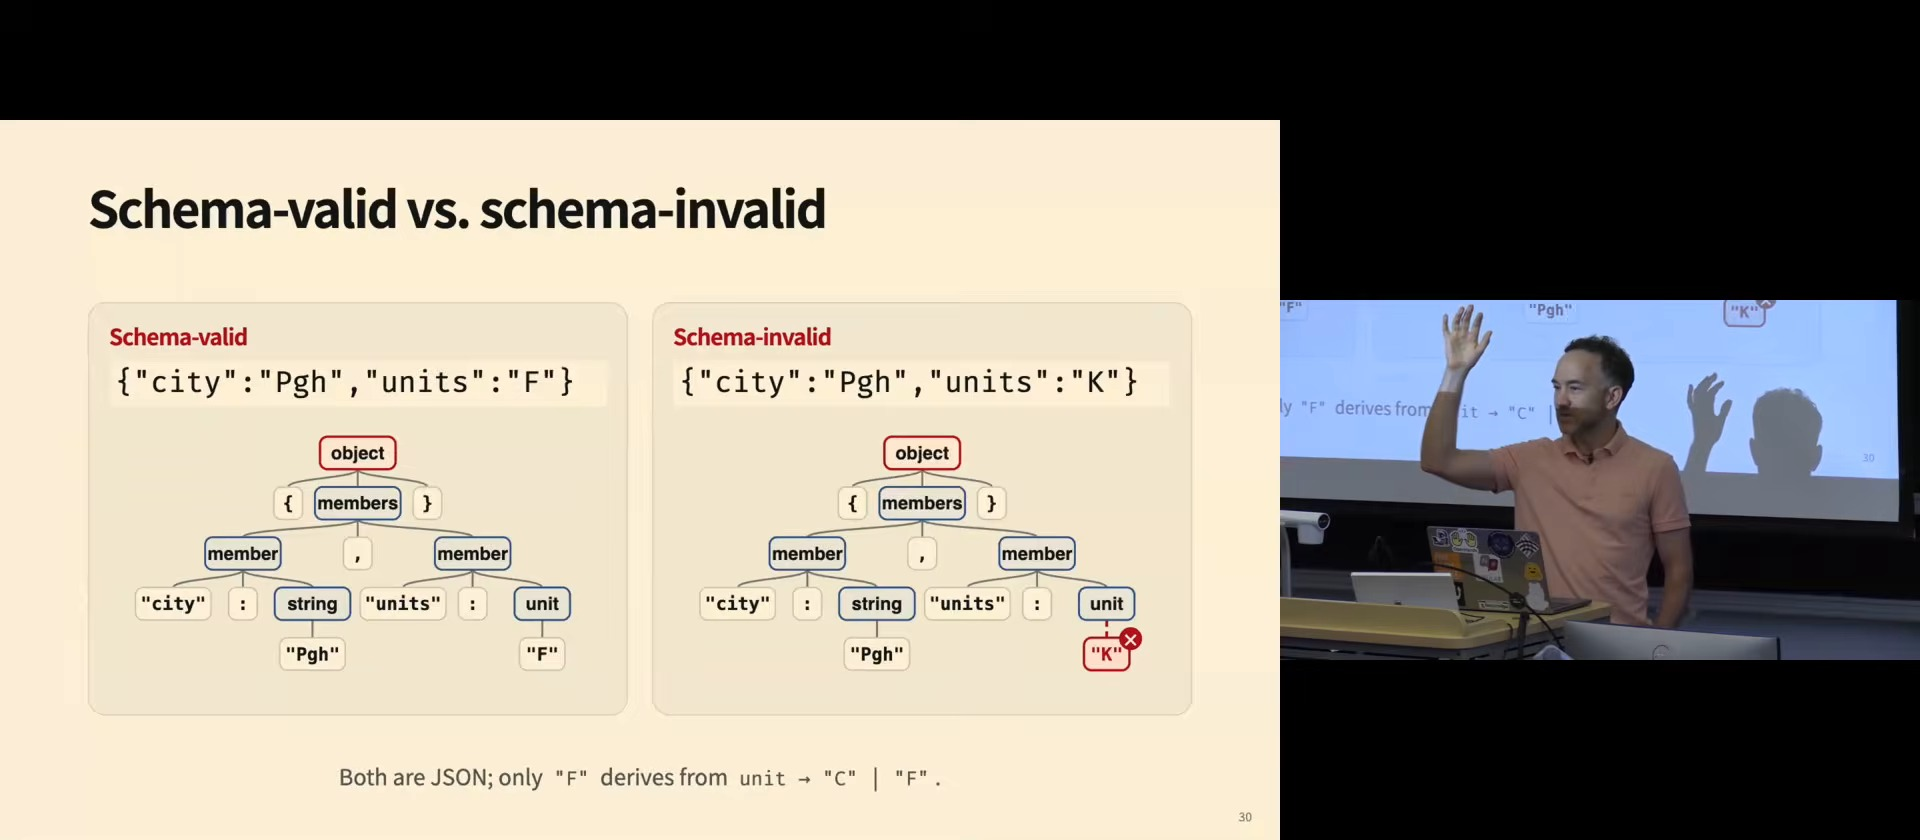
\includegraphics[width=\textwidth]{figures/fig_18_schema_tree.jpg}
\caption{schema 合法与非法：同一棵语法树上，\texttt{units:"K"} 在推导 unit 规则时无法归约\vtag}
\end{figure}
\srcnote{00:29:00--00:29:14}

理解这张图的关键是"归约"：合法的 JSON 可以被解析成一棵完整的语法树；非法输入并非"解析器报错"这么简单，而是在某个规则处无法完成归约——比如 \texttt{units} 的取值集合只允许 C 与 F，遇到 K 时那棵子树就长不出来。约束解码正是把这种"长不出来"变成生成时的硬约束。

\subsection{从正则到上下文无关文法}

讲者用一条递进的知识线解释了背后的计算理论：

\begin{itemize}
\item \textbf{正则表达式}对应\textbf{正则文法}，可以用\textbf{有限状态自动机}（FSA）解析：读一个 token 就转移一次状态。
\item \textbf{JSON Schema 不能}用正则文法表达（嵌套结构需要记忆），它对应的是\textbf{上下文无关文法}（CFG）。
\item CFG 需要一个带\textbf{栈}的自动机——\textbf{下推自动机}（PDA）：遇到数组/对象就 push，遇到闭合就 pop，栈负责记住"当前嵌套到了哪一层"。
\end{itemize}

\begin{figure}[H]
\centering
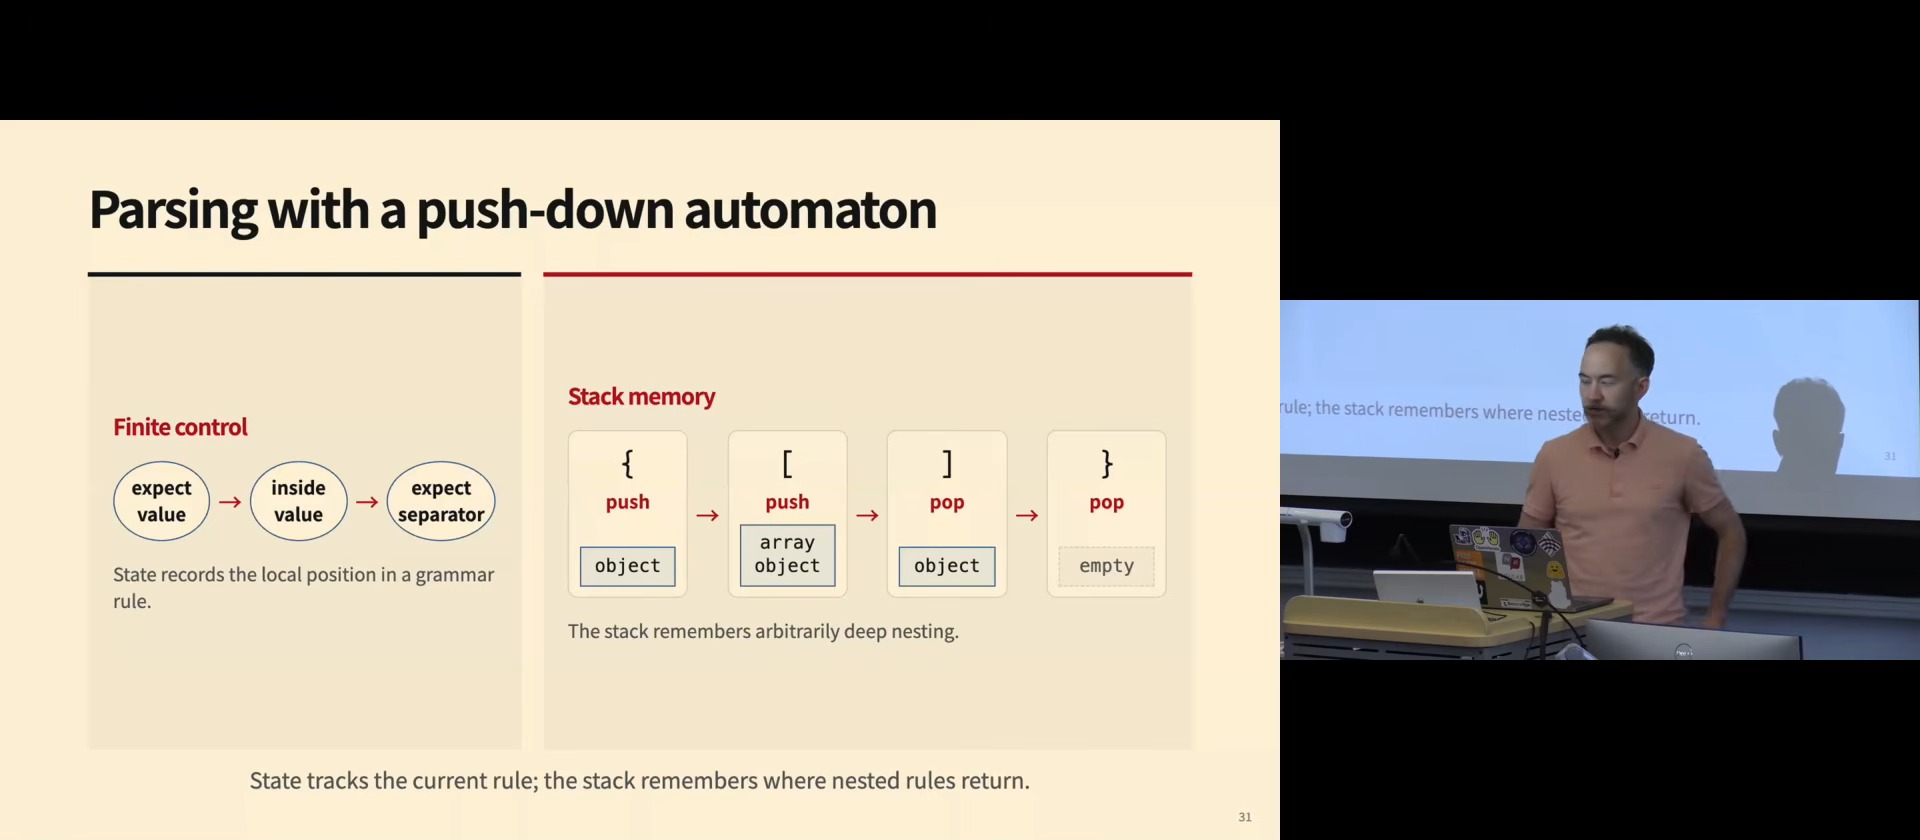
\includegraphics[width=\textwidth]{figures/fig_19_pushdown.jpg}
\caption{下推自动机：有限状态控制加一个栈，用 push/pop 记住嵌套结构在哪里闭合\vtag}
\end{figure}
\srcnote{00:32:00--00:32:14}

于是约束解码的流程是：把 JSON Schema 编译成 PDA；在生成过程中从左到右读取已产出的 token，让 PDA 的当前状态定义"下一步哪些 token 是合法的"。

\subsection{token masking：把非法 token 的概率清零}

具体实现只有两步：拿到模型输出的 logits 后，用结构给出的合法集合做一次逐 token 掩码（合法记 1、非法记 0），把非法位置置为负无穷，再 softmax 归一化到合法 token 上，最后采样。

\begin{equation}
p'_\theta(a \mid s) \;\propto\; p_\theta(a \mid s)\cdot \mathbb{1}\!\left[\,a \in \mathcal{L}(\mathcal{G})\,\right]
\end{equation}
式中 $s$ 为当前上下文，$a$ 为候选 token 序列，$\mathcal{G}$ 为从 JSON Schema 编译出的文法，$\mathcal{L}(\mathcal{G})$ 为它接受的合法序列集合，$\mathbb{1}[\cdot]$ 为指示函数。结果就是：\textbf{非法 token 的概率被彻底抹掉}，模型无法生成畸形调用。

\begin{figure}[H]
\centering
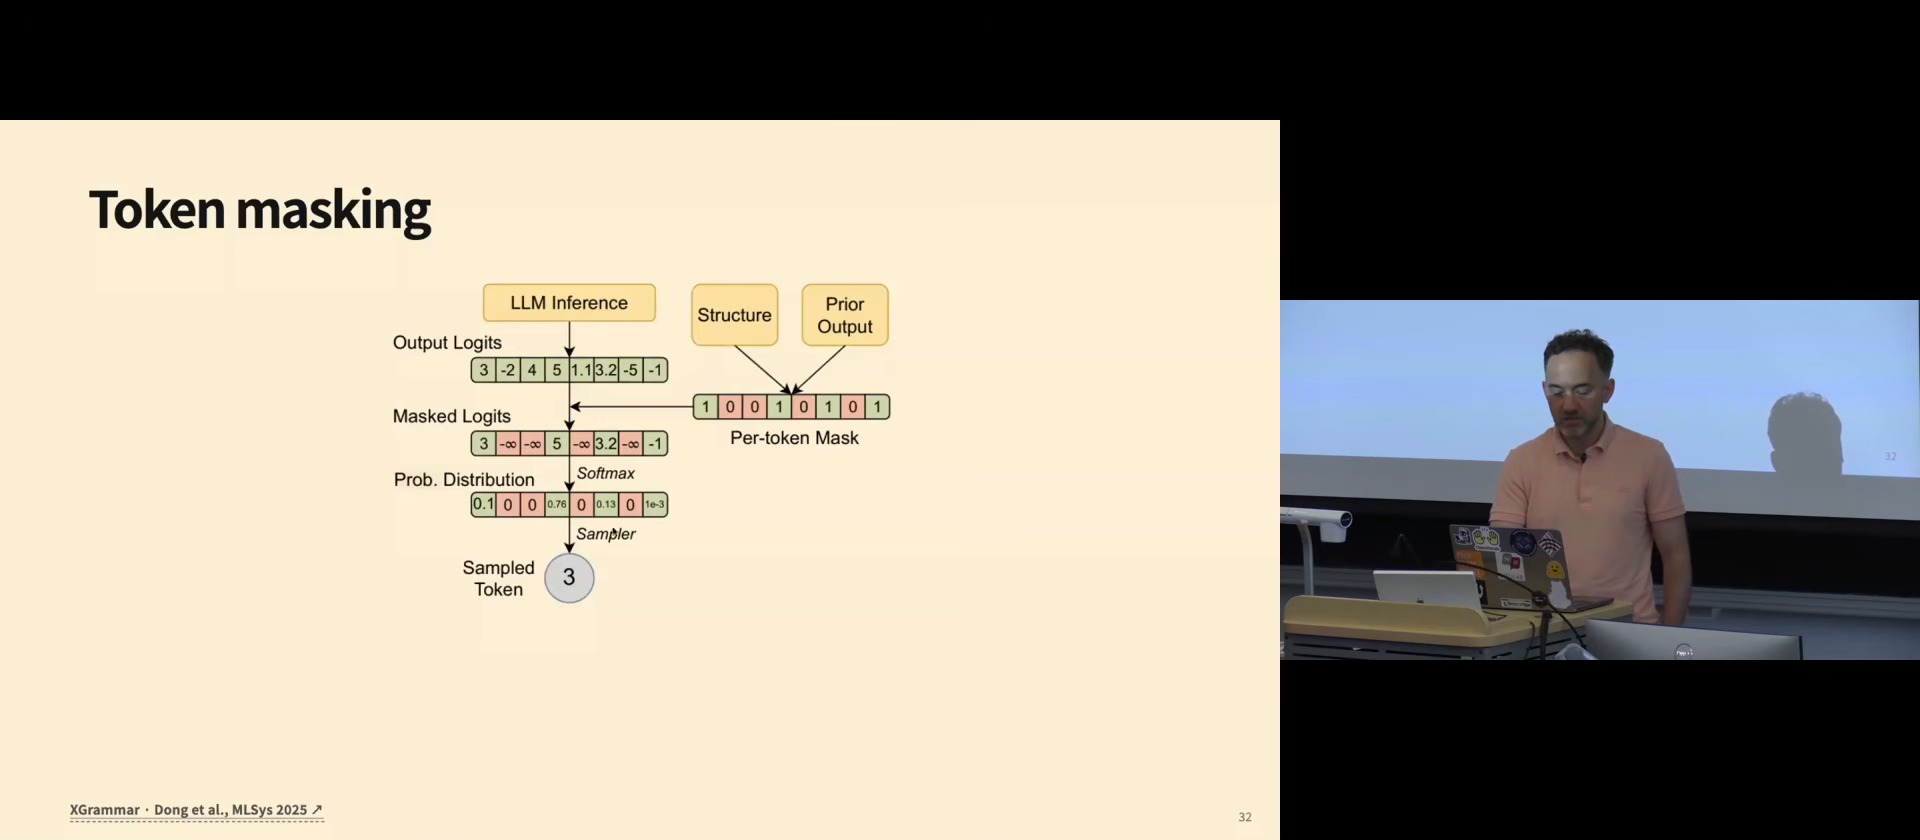
\includegraphics[width=\textwidth]{figures/fig_20_token_mask.jpg}
\caption{token masking 流水线：输出 logits → 逐 token 掩码 → 掩码后 logits → softmax → 采样\vtag}
\end{figure}
\srcnote{00:33:15--00:33:29}

工程上这一步不能太慢，否则会拖垮推理。XGrammar（由 CMU 机器学习系的同学开发、已在多家推理库中广泛使用）的做法很有代表性：把词表里的 token 预先分成"任何上下文都合法"与"任何上下文都非法"两类\textbf{离线预计算}，只有那些\textbf{依赖当前栈状态}的 token 才在线计算；同时把掩码生成与 LLM 推理引擎\textbf{重叠}执行，把开销藏起来。

\begin{figure}[H]
\centering
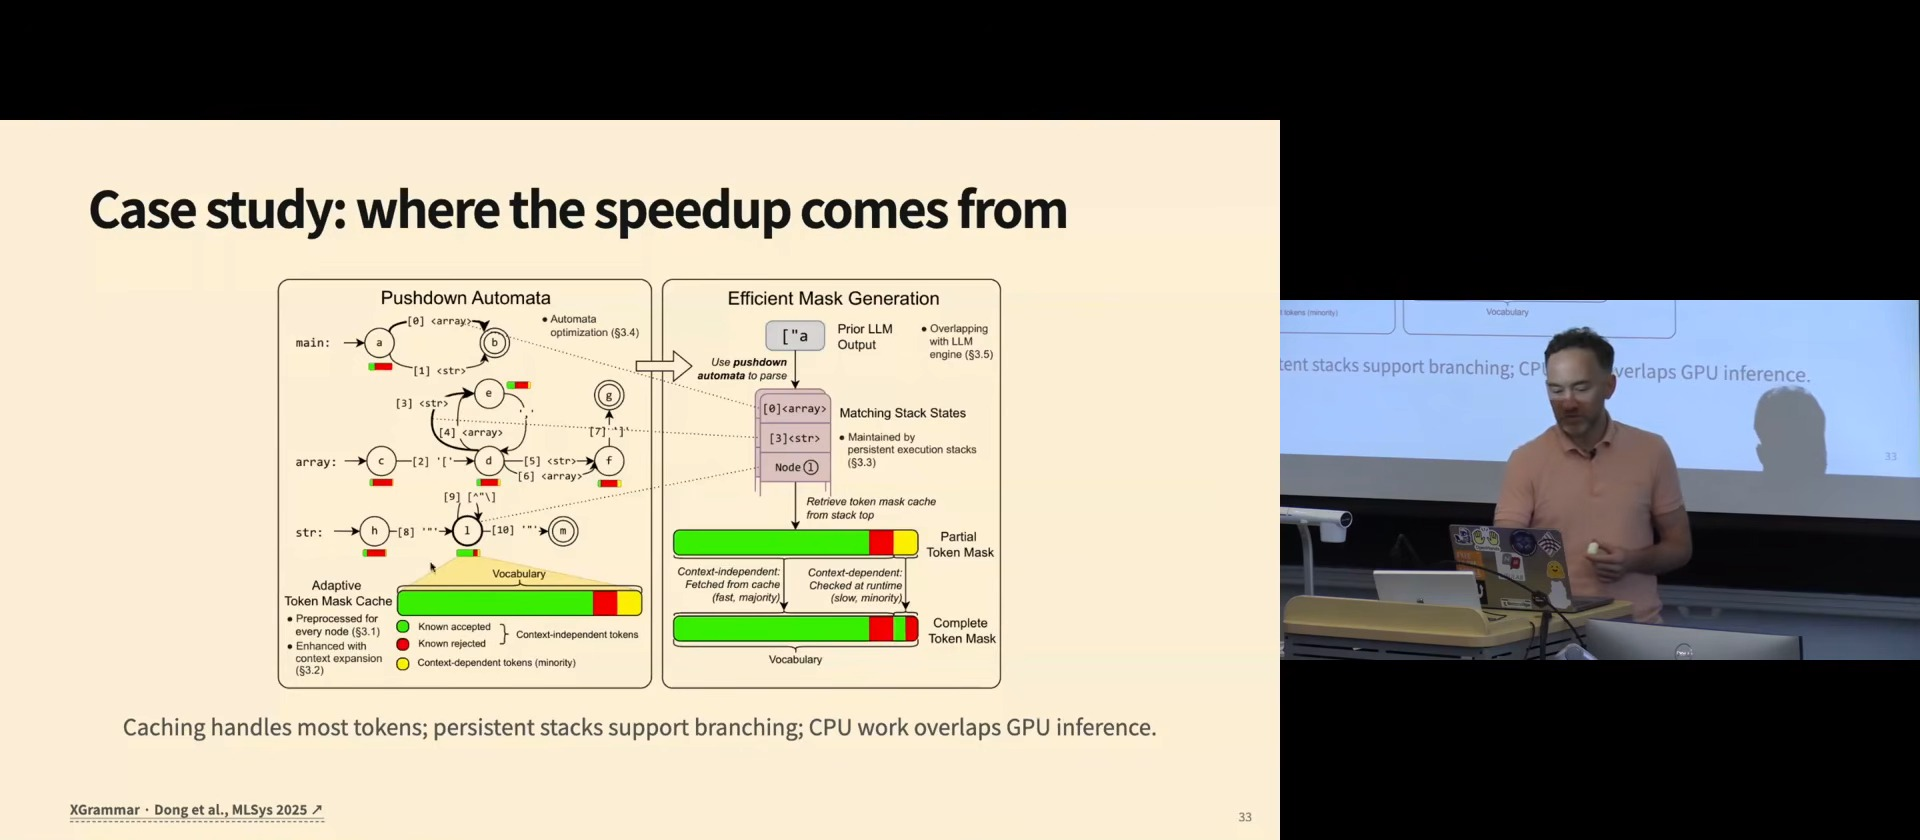
\includegraphics[width=\textwidth]{figures/fig_21_xgrammar.jpg}
\caption{XGrammar 案例：下推自动机 + 高效掩码生成（预计算多数 token）+ 与推理引擎重叠优化\vtag}
\end{figure}
\srcnote{00:35:00--00:35:14}

\begin{knowledgebox}{为什么这条知识值得学}
约束解码不是"某个库的黑魔法"，而是三样东西的组合：JSON Schema（表达约束）、上下文无关文法与下推自动机（把约束变成状态机）、logits 掩码（把状态机接进采样）。理解了它，就能判断一个推理服务"是否支持结构化输出"到底意味着什么——以及为什么不同供应商的调用成功率会差出两个数量级。
\end{knowledgebox}

\subsection{唯一失效的场景}

即使开了约束解码，仍有一种情况会产出不合法调用：\textbf{输出被 max tokens 截断}。此时模型还在合法路径上，但没走到接受状态，于是你会得到半截 JSON。讲者的处理建议是提前预估"完成这次调用还差多少 token"，并在预算不足时截断或重试——他在课上把实现这个功能当成"额外加分作业"抛给了学生。

\begin{warningbox}{约束不等于正确}
约束解码只解决语法层：它不检查这次调用是否该发生、参数值是否真实、是否有权限。一个 schema 完全合法的 \texttt{delete\_all()} 依然是灾难——所以还需要校验、权限与沙箱这三层（下一节与后续安全讲座）。
\end{warningbox}

\subsection{本章小结}
约束解码把"格式合法"从概率问题变成结构问题：JSON Schema → 上下文无关文法 → 下推自动机 → logits 掩码。它几乎消灭了畸形调用，但不约束语义与权限。下一节转向接口层：这些工具究竟以什么形式被"挂"到 agent 上。

\section{接口形态：进程内、REST 与 MCP}

\subsection*{本节回答的问题}
同样是调用外部能力，进程内库、REST API 与 MCP 各自是什么契约？MCP 存在的真正理由是什么？

\subsection{从进程内函数到网络服务}

最轻的形态是进程内库：\texttt{weather\_lib.py} 里的函数与调用者共享一个进程，靠 Python 的导入机制提供编程接口，不涉及网络与凭证。这种形态简单，但只适合同一台机器、同一套权限的场景。

\begin{figure}[H]
\centering
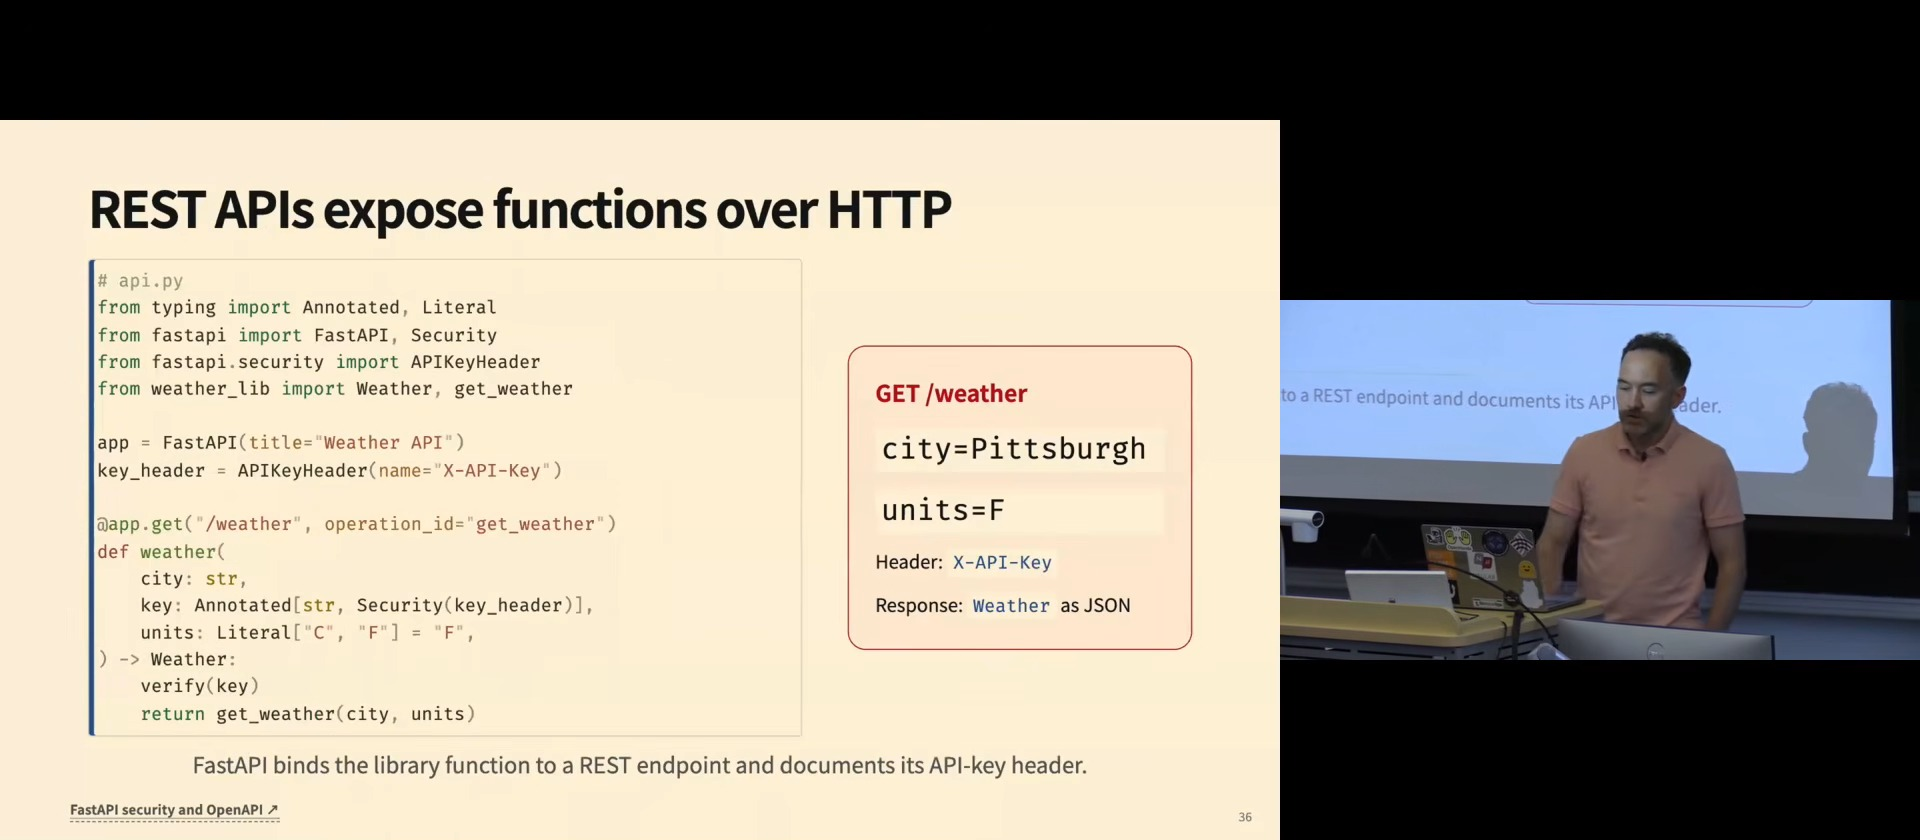
\includegraphics[width=\textwidth]{figures/fig_22_fastapi.jpg}
\caption{REST：用 FastAPI 把进程内函数暴露成 HTTP 接口，并加上 API key 鉴权\vtag}
\end{figure}
\srcnote{00:36:45--00:36:59}

把它变成 REST API 只需要一个装饰器与一个密钥头：FastAPI 会把参数与返回值变成\textbf{OpenAPI 描述}（内含 JSON Schema），这份描述可以原样喂给模型作为工具定义；同时 API key 让服务端可以拒绝未授权调用。讲者列出 REST 路线的三个要点：读 OpenAPI 文档获得接口、构造 HTTP 请求（例如 \texttt{curl}）、限制凭证的暴露范围。对能跑 bash 的 coding agent 来说，\texttt{curl} 本身就是一种"工具调用"。

\begin{knowledgebox}{FastAPI 的两个"免费"好处}
一是鉴权：服务端可以要求 API key，从而阻止未授权访问；二是\textbf{JSON Schema 免费得到}——接口定义即工具定义，不需要再手写一份 schema。这也是讲者推荐用 FastAPI 做工具服务的原因：接口即文档、文档即提示。
\end{knowledgebox}

\subsection{MCP：一种"agent 专用"的接口契约}

讲者坦言自己第一次看到 MCP（Model Context Protocol，Anthropic 提出）时的反应是："既然已经有 REST，为什么还要多一层？"随后的分析给出了 MCP 真正的两个理由。

第一是\textbf{结构}：MCP 把系统分成 host（AI 应用）、client 与 server，本地用 stdio、远程用 HTTP 连接；host 里可以挂多个 client，每个 client 连一个 server（文件系统、Sentry 等）。它把"发现与调用能力"这件事标准化了。

\begin{figure}[H]
\centering
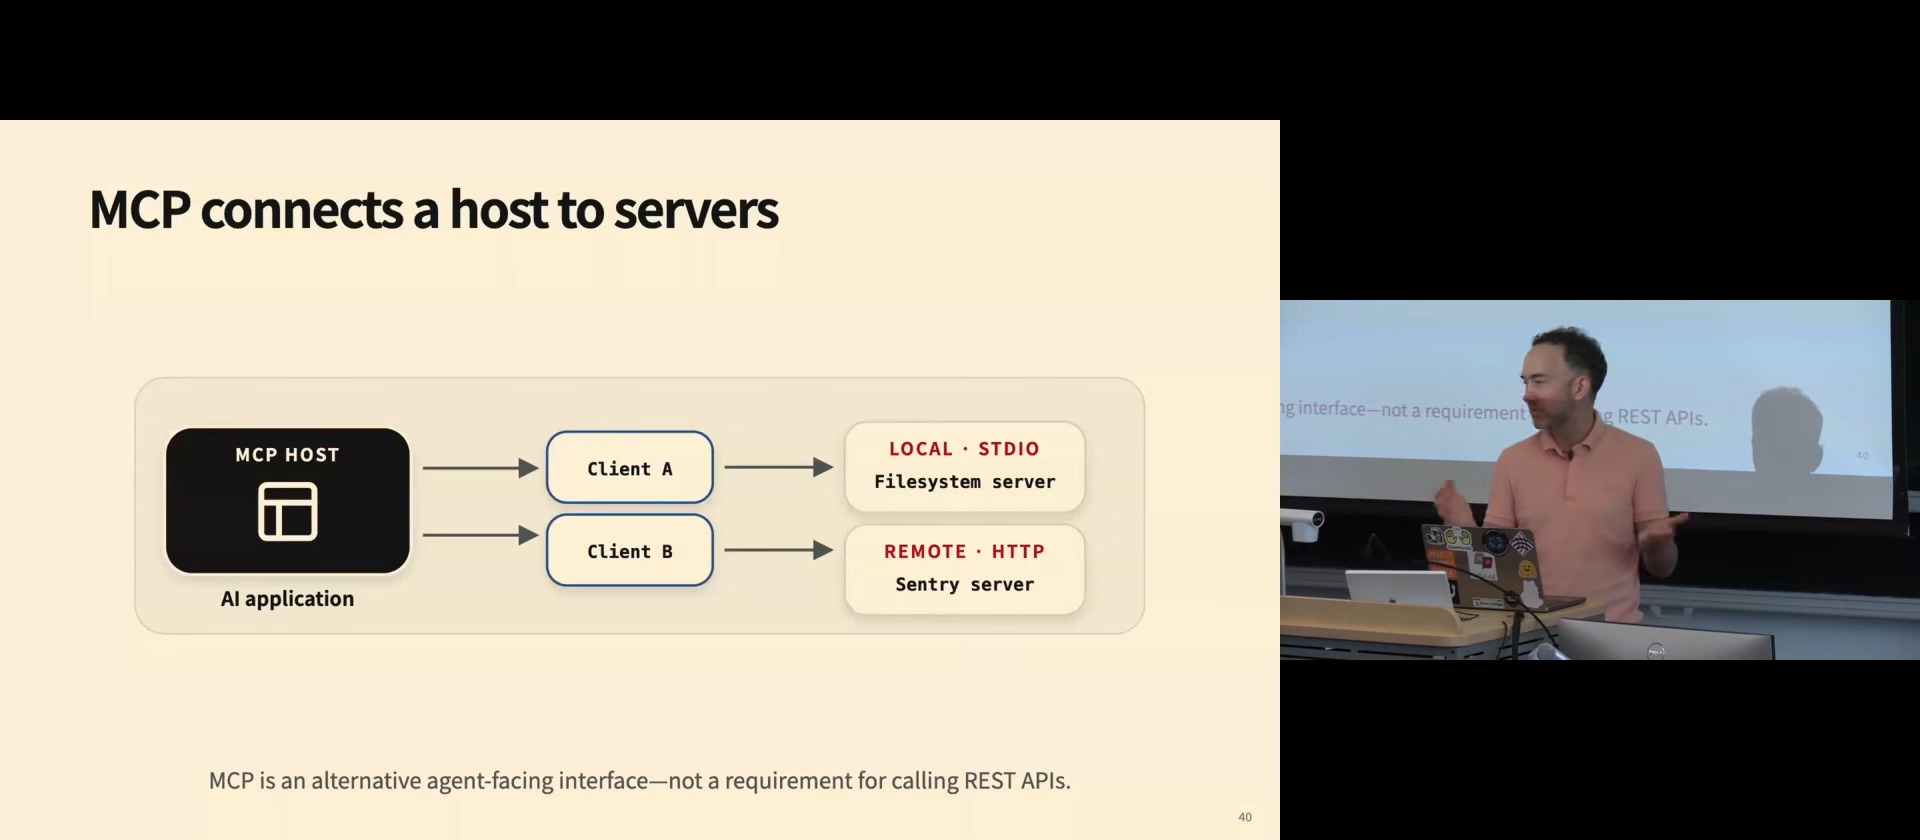
\includegraphics[width=\textwidth]{figures/fig_23_mcp_diagram.jpg}
\caption{MCP：host 通过多个 client 连接 server（本地 stdio / 远程 HTTP），把能力发现与调用标准化\vtag}
\end{figure}
\srcnote{00:40:30--00:40:44}

第二，也是更重要的，是\textbf{凭证隔离}：MCP server 持有上游 API key（例如你的 GitHub token），agent 只拿到 MCP 自己的 key。这样即使 agent 出于某种原因把凭据泄露出去，泄露的是权限受限的 MCP key，而不是能改你所有仓库的 GitHub token。讲者用一句话点出动机：\textbf{给 agent 的东西应当是"即使泄漏也相对无害"的}。

\begin{figure}[H]
\centering
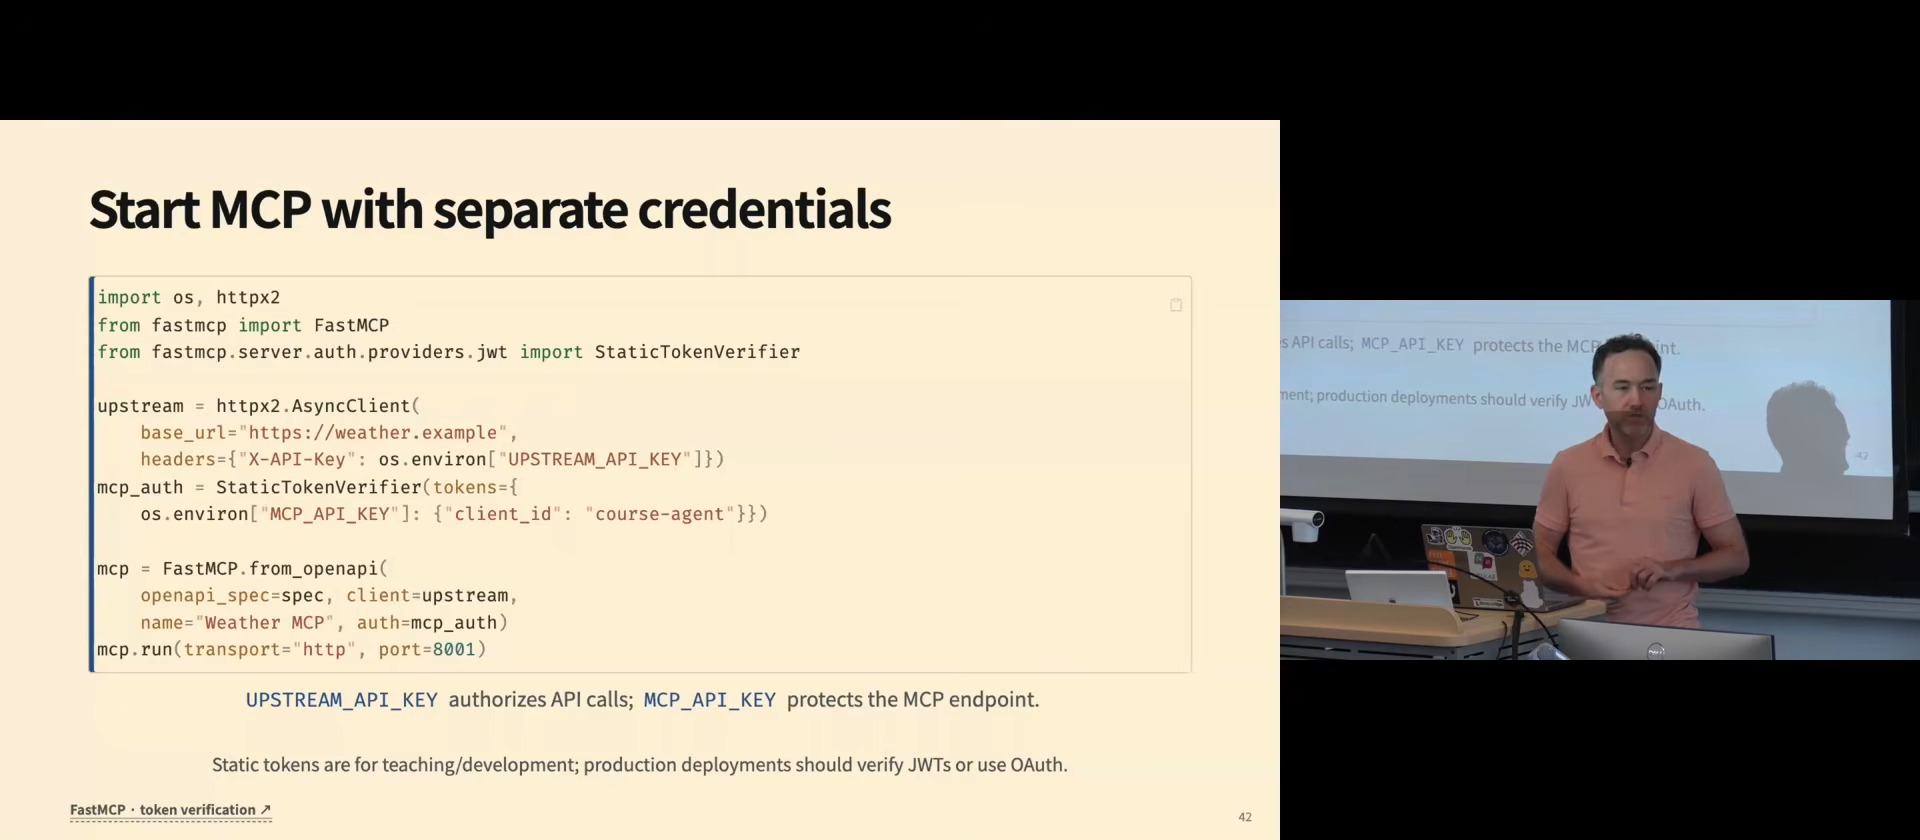
\includegraphics[width=\textwidth]{figures/fig_24_mcp_creds.jpg}
\caption{MCP 独立凭证：上游 secret 留在 server；agent 只拿 MCP key，泄漏的后果被限制\vtag}
\end{figure}
\srcnote{00:41:30--00:41:44}

此外 fastMCP 让写 MCP server 像写 FastAPI 一样简单，甚至可以把现成的 OpenAPI 描述转成 MCP 工具；官方有 MCP registry，社区也有大量按热度排序的 server 目录。

\begin{figure}[H]
\centering
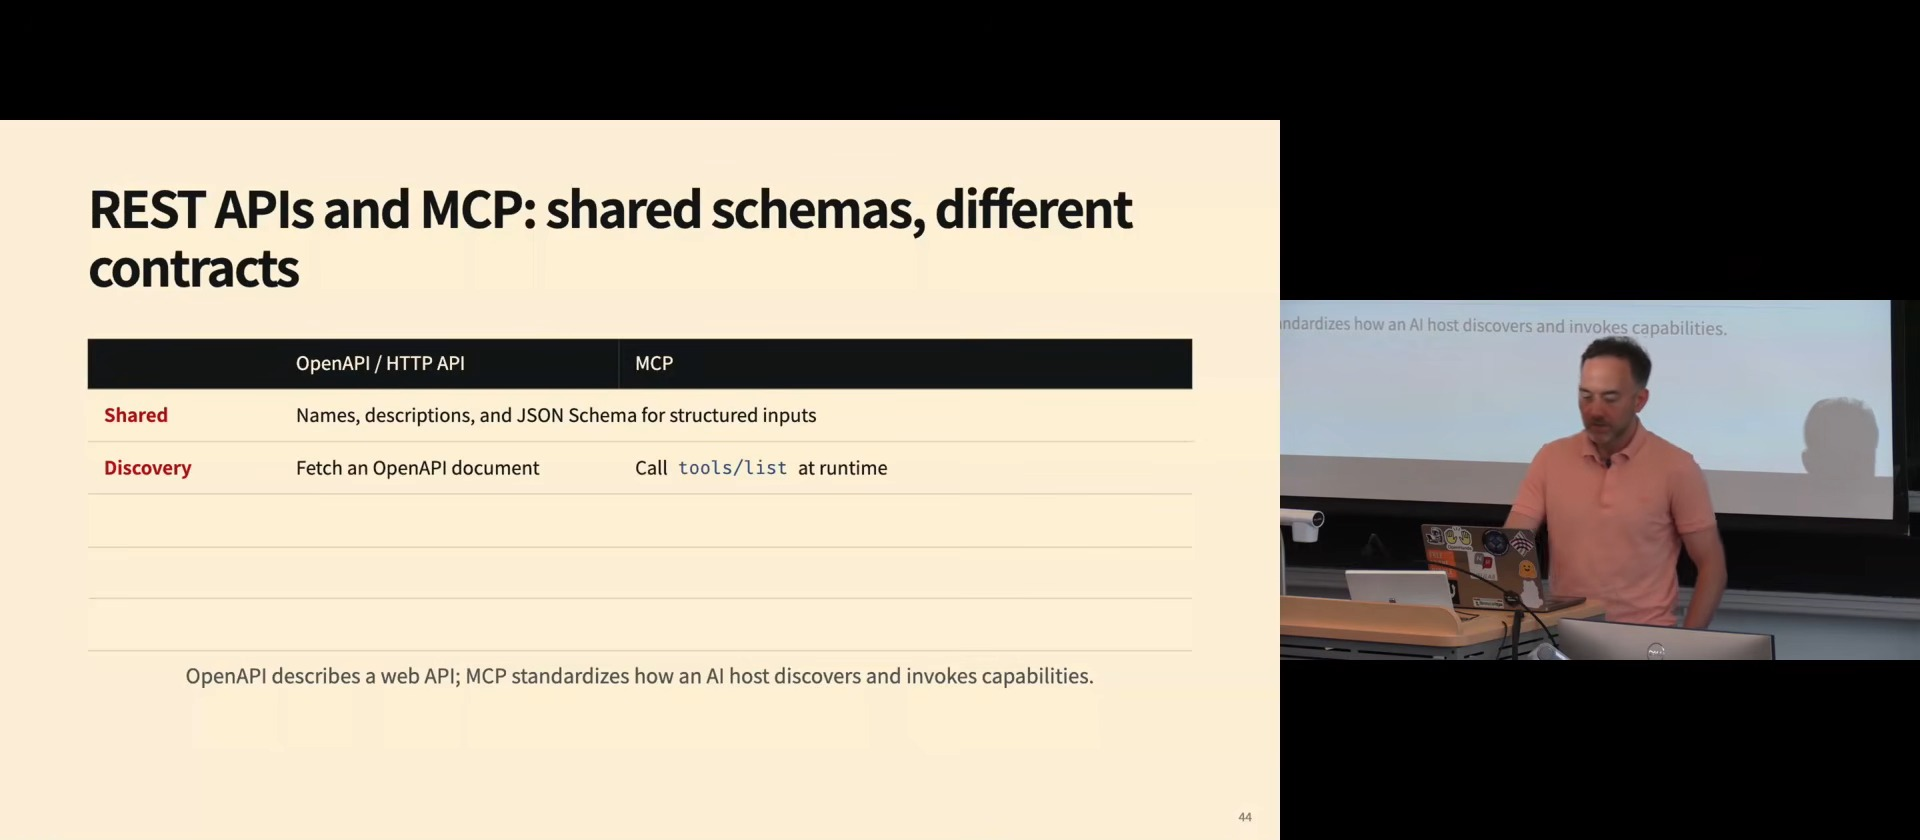
\includegraphics[width=\textwidth]{figures/fig_25_rest_vs_mcp.jpg}
\caption{REST 与 MCP：共享名字、描述与 JSON Schema；差异在发现方式、调用传输与认证契约\vtag}
\end{figure}
\srcnote{00:43:00--00:43:14}

\begin{center}
\small
\begin{tabular}{lll}
\toprule
维度 & OpenAPI / HTTP API & MCP \\
\midrule
共享 & 名字、描述、结构化输入的 JSON Schema & 同左 \\
发现 & 读 OpenAPI 文档 & 专用的 list tools 接口 \\
调用 & 发 HTTP 请求 & 走 MCP transport（stdio / socket） \\
认证 & API key / token 直接给调用方 & MCP key 与 upstream key 分离 \\
附加 & 无 & resources、prompts、extensions \\
\bottomrule
\end{tabular}
\end{center}

\begin{importantbox}{选型的判断顺序}
\textbf{（1）}同一台机器、同一权限域 → 进程内库最省事；\textbf{（2）}要跨机器、要鉴权、要复用生态 → REST + OpenAPI；\textbf{（3）}需要把上游凭证与 agent 隔离、或要接现成的 MCP 生态 → MCP。三者的工具定义可以共享同一份 JSON Schema，真正不同的是\textbf{调用与信任的边界}。
\end{importantbox}

\subsection{本章小结}
接口形态决定的不只是"能不能调"，更是"凭证握在谁手里、泄漏后损失多大"。下一节处理另一类工程问题：当一次任务需要多次互不依赖的调用时，如何用并行把等待时间压下来。

\section{并行工具调用与效率悖论}

\subsection*{本节回答的问题}
并行调用能省多少时间、前提是什么、怎么实现？为什么更贵的模型按任务算反而可能更便宜？

\subsection{串行与并行的成本差}

幻灯片把同一组调用（查询天气、日历、航班并生成结果）按两种方式计时。串行时每个调用都要等前一个结束，且每次都要重新生成一次，总耗时约 6.4 秒；并行时模型在一轮生成里发出三个独立调用，只等最慢的那个返回，总耗时约 2.8 秒。

\begin{equation}
T_{\text{serial}} \;=\; \sum_{i=1}^{n}\bigl(g_i + e_i\bigr),
\qquad
T_{\text{parallel}} \;=\; g \;+\; \max_{i} e_i
\end{equation}
式中 $g_i$ 为第 $i$ 轮模型生成耗时，$e_i$ 为第 $i$ 个工具执行耗时；并行场景下所有调用共享一次生成 $g$，等待时间由最慢的工具决定。代入幻灯片数字（约 $2\times0.8+\max(1.2,0.9,1.1)\approx2.8$ 秒）就能看出：\textbf{并行的收益来自"少生成几轮"而不只是"同时执行"}。

\begin{figure}[H]
\centering
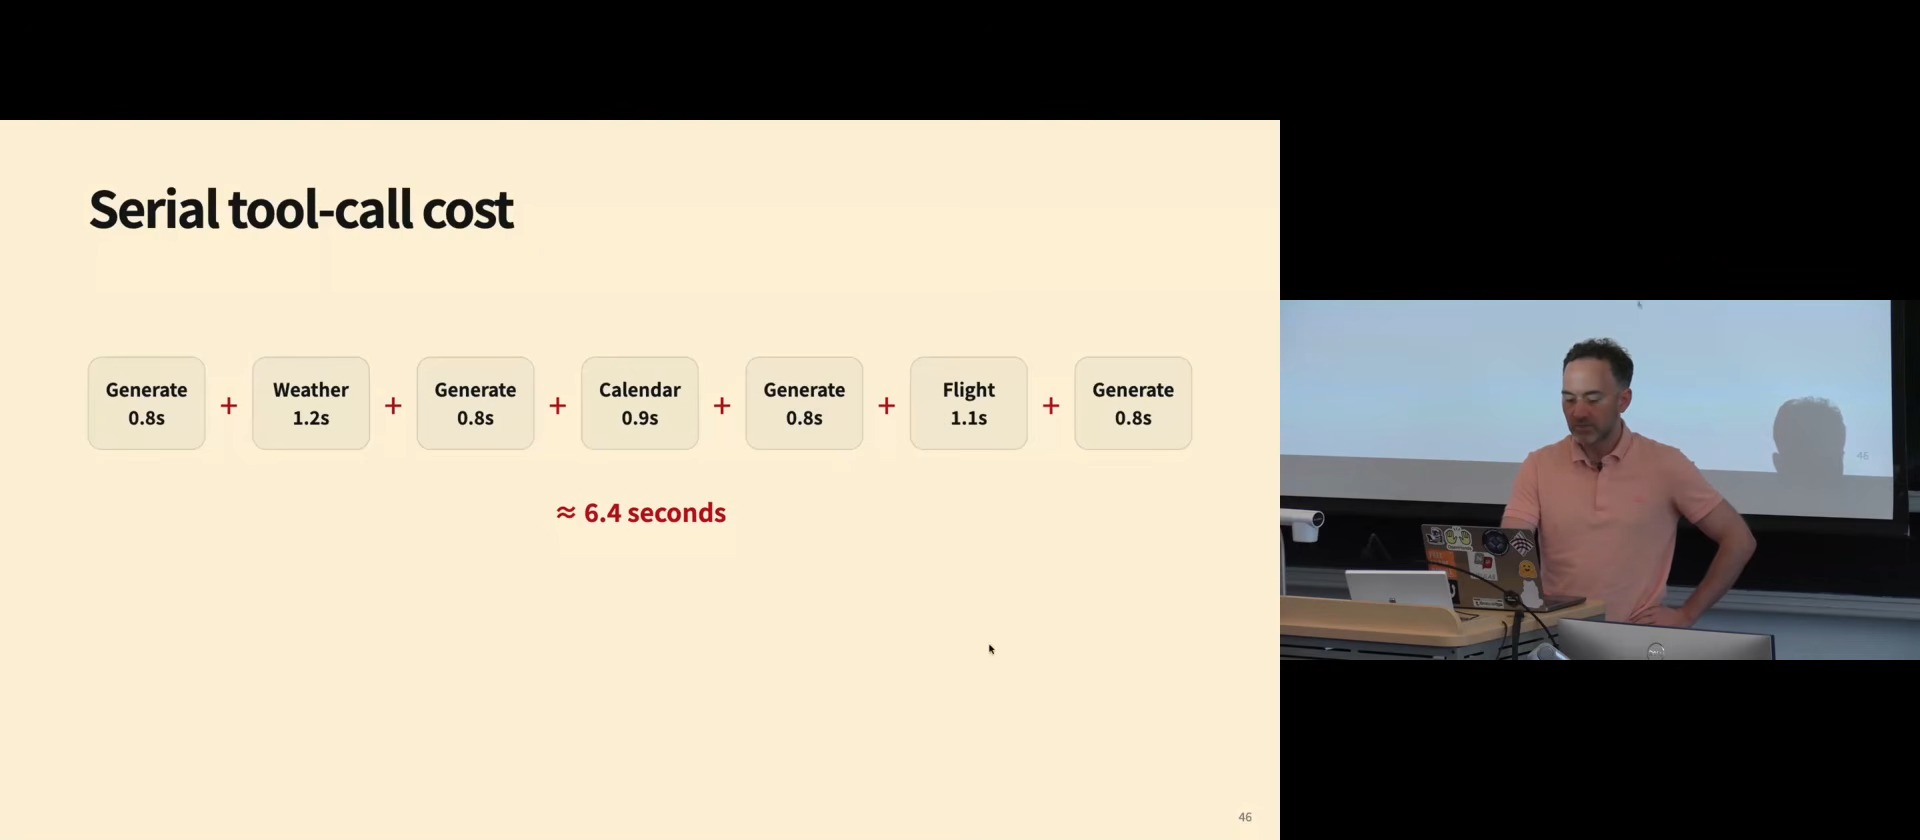
\includegraphics[width=\textwidth]{figures/fig_26_serial_cost.jpg}
\caption{串行成本：weather/calendar/flight 逐次调用并逐次生成，合计约 6.4 秒\vtag}
\end{figure}
\srcnote{00:45:30--00:45:44}

\begin{figure}[H]
\centering
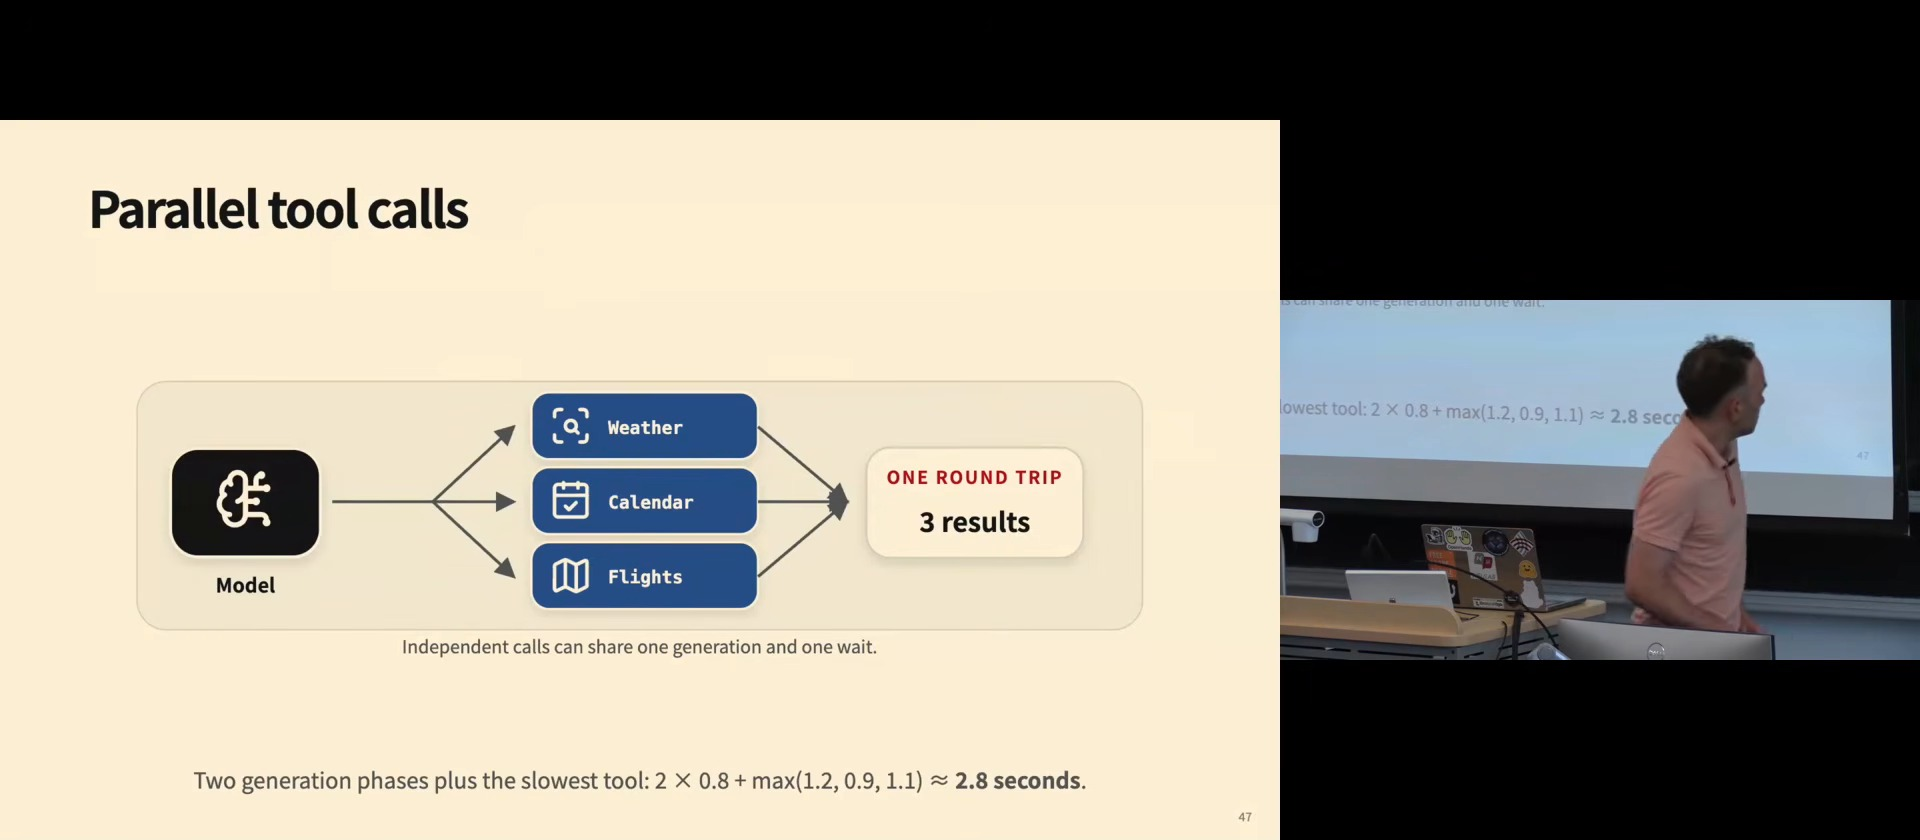
\includegraphics[width=\textwidth]{figures/fig_27_parallel_cost.jpg}
\caption{并行调用：一次生成 + 一次等待（取最慢者），同一任务约 2.8 秒\vtag}
\end{figure}
\srcnote{00:45:45--00:45:59}

\subsection{前提：只并行独立调用}

并行不是免费的午餐。幻灯片把调用分成两列：可以安全并行的（查天气、读日历、查航班）与必须排序的（先查客户 ID，再用 ID 取订单，再退款）。判断标准只有一条：\textbf{后一个调用的参数是否依赖前一个的结果}。

\begin{figure}[H]
\centering
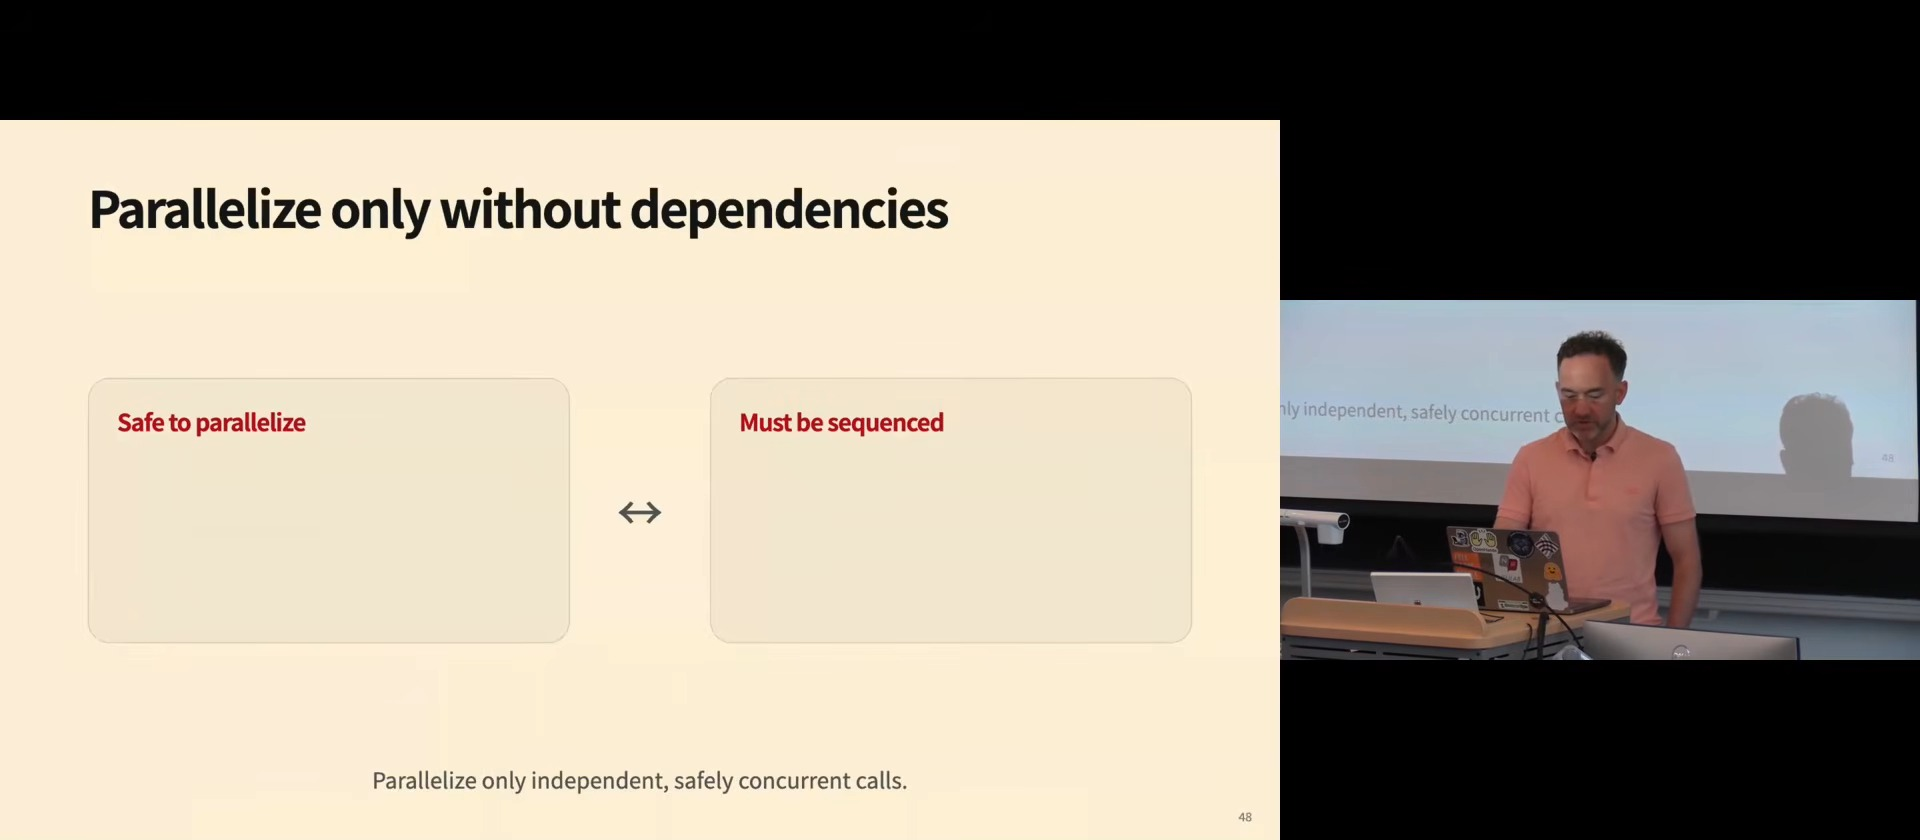
\includegraphics[width=\textwidth]{figures/fig_28_dependency.jpg}
\caption{并行边界：只有彼此独立、可安全并发的调用才能并行；有依赖的调用必须排序\vtag}
\end{figure}
\srcnote{00:46:00--00:46:14}

实现上没有魔法：把一批调用交给 \texttt{asyncio.gather}，用 call ID 收回每个结果，再拼回一条历史。

\begin{lstlisting}[language=Python, caption=并发执行一批工具调用（幻灯片摘录：按 call ID 收结果）]
async def execute(call):
    args = json.loads(call.arguments)
    value = await TOOLS[call.name](**args)
    return call.call_id, value

results = await asyncio.gather(
    *(execute(call) for call in function_calls)
)
\end{lstlisting}

\begin{importantbox}{并行调用的三个约束}
\textbf{（1）数据依赖}：有依赖必须串行；\textbf{（2）副作用}：两个都会修改同一状态的调用不能并行（顺序会改变结果）；\textbf{（3）失败处理}：并行组里一个失败，其余结果仍要按 call ID 回填，否则 history 不完整（见第 3 章最后的警告）。
\end{importantbox}

\subsection{效率悖论：更贵的模型可能更便宜}

讲者提出一个反直觉的观察：如果按\textbf{单个任务的完成成本}衡量，更贵的模型有时反而更便宜。原因有两个：其一，更强的模型更快找到正确解法，少走弯路；其二，新模型\textbf{并行工具调用}能力强得多——一次输出多个调用（同时看多张图、同时改多个文件），把轮数压下来。

课堂上有人问：并行调用的机制早就存在，为什么最近才普及？学生的回答被讲者确认："是强化学习逼出来的。"当训练目标里对\textbf{任务耗时/冗长度}施加惩罚时，并行调用是最直接的省时手段，于是模型学会了它。这条观察也解释了为什么"能力"与"效率"在 agent 场景里往往不是两件事。

\begin{knowledgebox}{给读者的成本观}
选模型不要只看单价：要按"每个成功任务的成本"算——包含轮数、token 数、失败重试与人工介入。一个单价高一倍、但把 10 轮压成 3 轮的模型，总账常常更便宜。这与第 1 讲"更贵的模型可能更划算"是同一个判断在两个场景下的体现。
\end{knowledgebox}

\subsection{本章小结}
并行调用把"多次生成 + 多次等待"压成"一次生成 + 一次等待"，前提是调用之间互不依赖；它还能解释"贵模型更便宜"这一反常现象。最后一节转向评测：工具调用做得好不好，究竟看哪些指标。

\section{评测工具使用}

\subsection*{本节回答的问题}
工具调用能力该用什么基准衡量？评测为什么不能只看端到端成功率，供应商差异又从哪来？

\subsection{Berkeley Function Calling Leaderboard}

讲者先区分了两件事：\textbf{端到端 agent 任务}的评测（后面再讲）与\textbf{工具可用性}的评测。后者是前者的前提——如果模型连调用都写不对，端到端成功率必然上不去。

最常被引用的基准是 Berkeley Function Calling Leaderboard（BFCL），它经历了四个版本：V1 只做单轮调用，之后逐步覆盖多轮、agentic 与 robustness。单轮维度考察 \texttt{simple}、\texttt{multiple}、\texttt{parallel} 与 \texttt{multiple-parallel}；多轮维度覆盖缺少函数、缺少参数、长上下文等；agentic 维度涉及 web search 与 memory；robustness 维度专门测\textbf{参数幻觉}与\textbf{格式敏感性}——后者正是本讲第 3 章讲的"各模型协议不同"。

\begin{figure}[H]
\centering
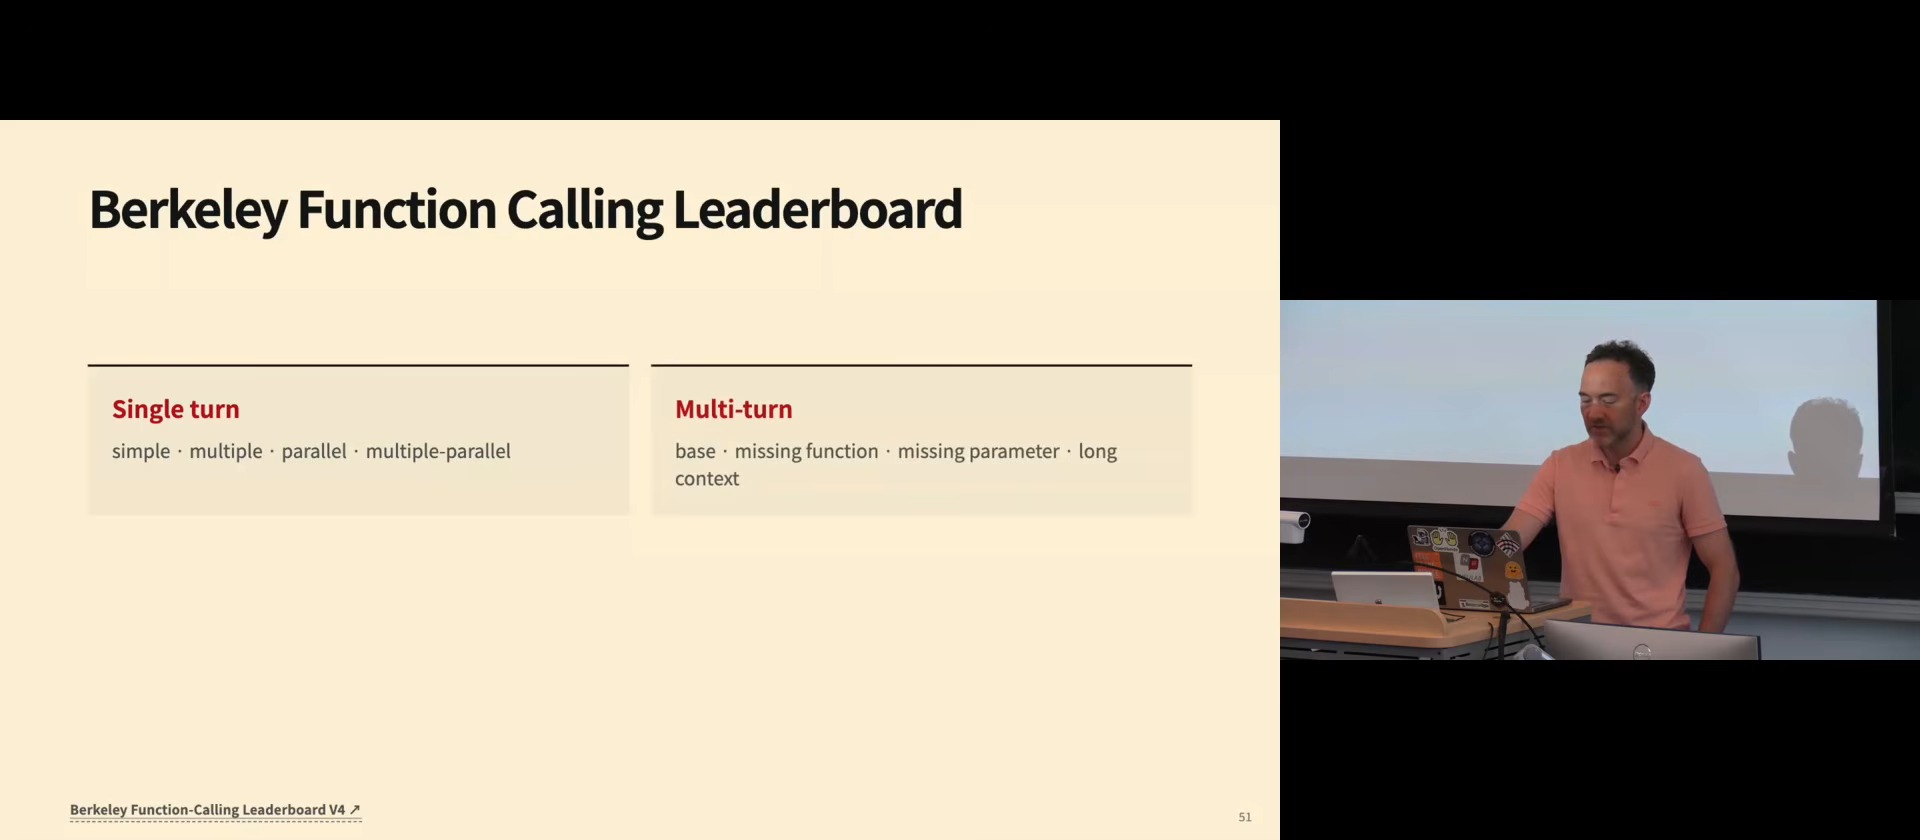
\includegraphics[width=\textwidth]{figures/fig_29_bfcl.jpg}
\caption{BFCL V4 的四个维度：单轮 / 多轮 / agentic / robustness（含参数幻觉与格式敏感性）\vtag}
\end{figure}
\srcnote{00:49:30--00:49:44}

\subsection{评测整条栈}

只给一个"任务成功了吗"的分数太粗，幻灯片把评测拆成四层，并指出每层的典型失败与指标：

\begin{center}
\small
\begin{tabular}{lll}
\toprule
层次 & 问题 & 典型失败 / 指标 \\
\midrule
Selection & 选对工具了吗 & 漏调、多调；precision / recall \\
Arguments & 参数值对吗 & 字段或取值错误；参数级准确率 \\
Order（agentic） & 顺序对吗 & 依赖被颠倒；步骤级检查 \\
Execution & 端到端成功了吗 & 需要真实执行环境 \\
\bottomrule
\end{tabular}
\end{center}

\begin{figure}[H]
\centering
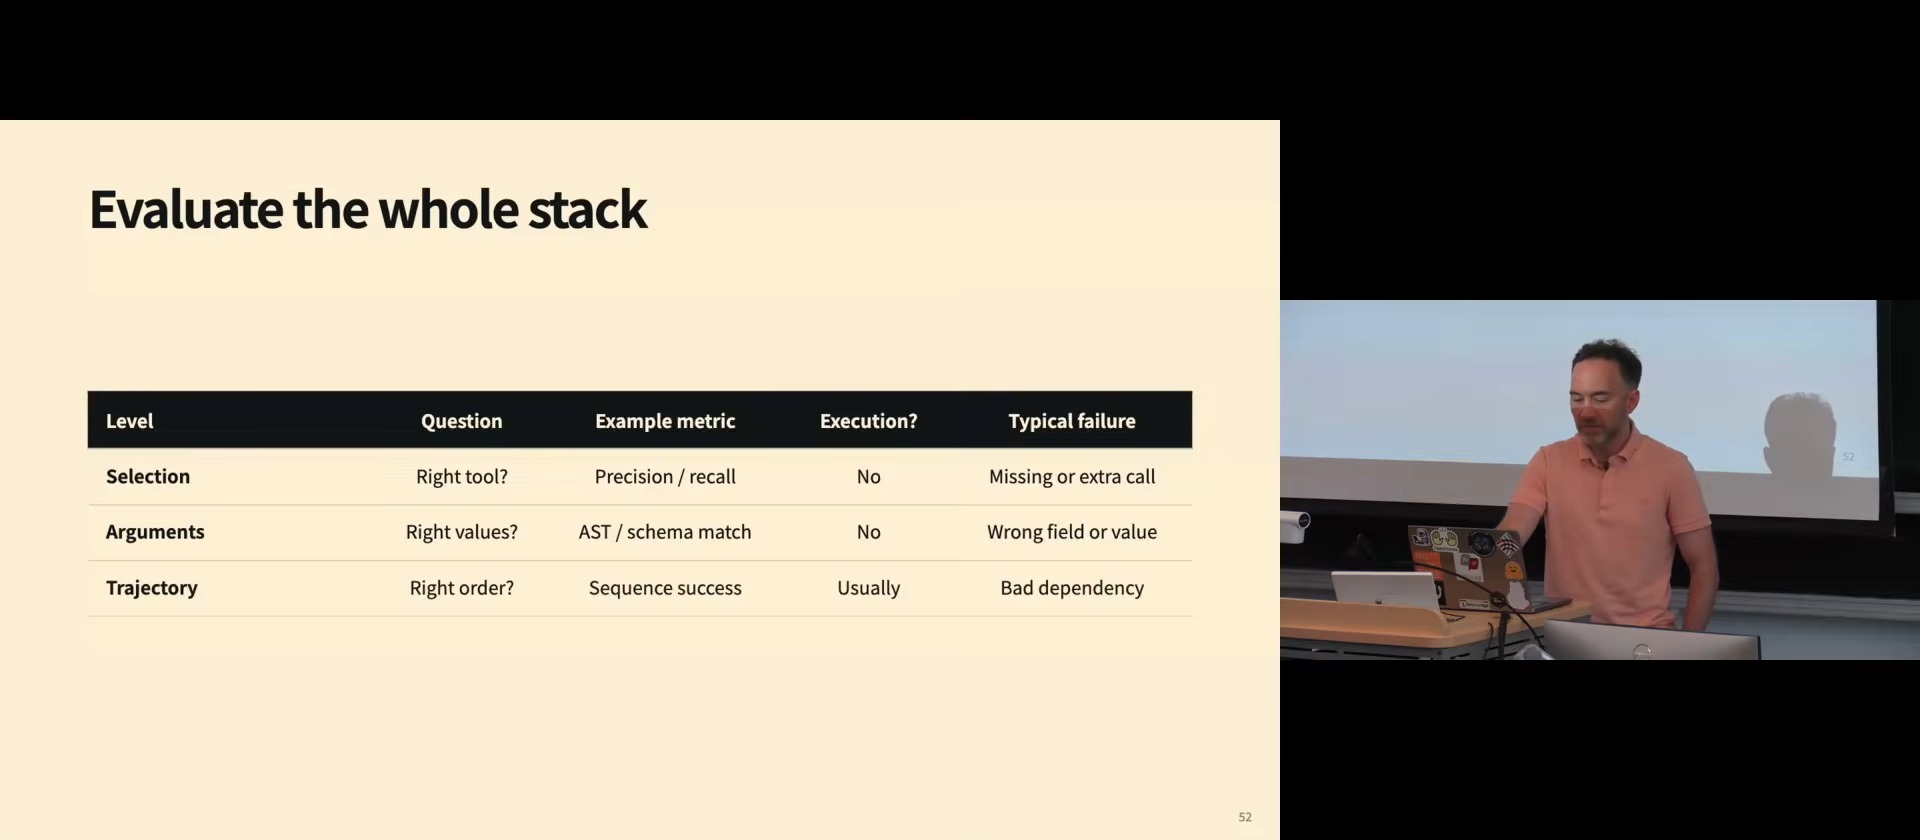
\includegraphics[width=\textwidth]{figures/fig_30_eval_stack.jpg}
\caption{评测整条栈：从"选对工具"到"端到端执行"，每层的失败模式与指标都不同\vtag}
\end{figure}
\srcnote{00:50:00--00:50:14}

\subsection{质量的运行维度}

幻灯片进一步提醒：一个\textbf{正确}的 agent 也可能无法使用。质量除了正确性，还有三个运行维度：\textbf{效率}（延迟、调用次数、token、成本）、\textbf{可靠性}（超时、重试、部分失败——"在真实供应商行为下报告任务成功率"）、\textbf{安全}（策略、权限、副作用）。这三个维度在不同版本的 BFCL 里逐步被纳入。

\begin{figure}[H]
\centering
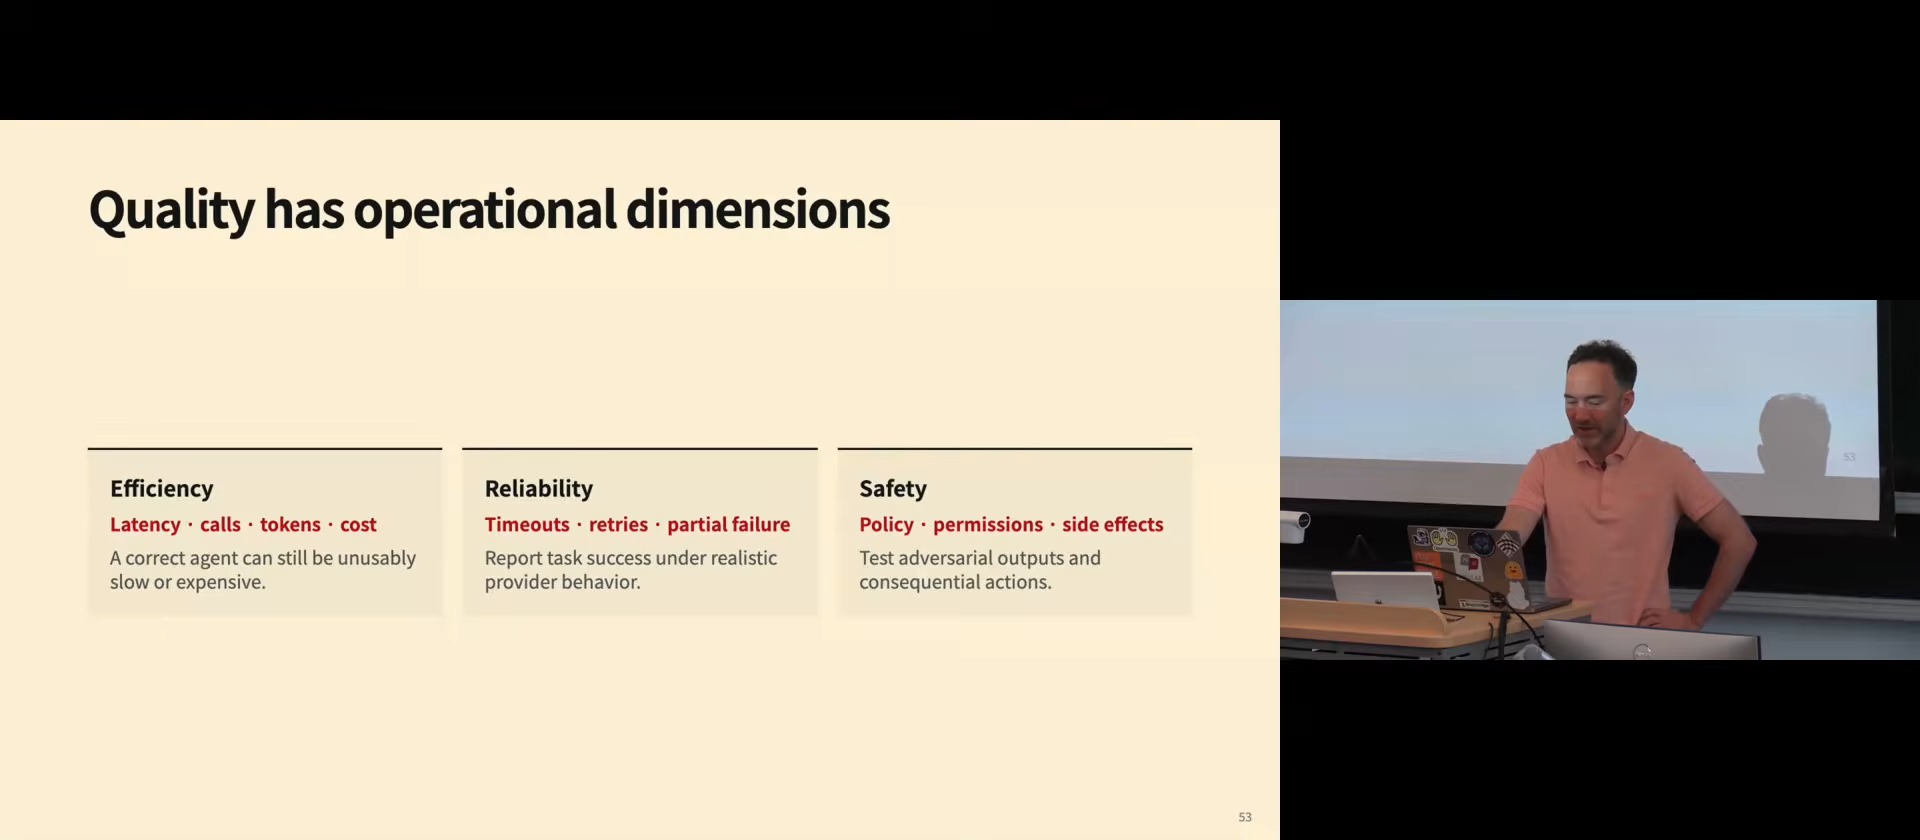
\includegraphics[width=\textwidth]{figures/fig_31_quality_dims.jpg}
\caption{质量的运行维度：效率（延迟/调用数/token/成本）、可靠性（超时/重试/部分失败）、安全（策略与副作用）\vtag}
\end{figure}
\srcnote{00:51:15--00:51:29}

\begin{importantbox}{评测清单}
一个可用的工具调用评测至少回答四件事：\textbf{选得对不对}（selection）、\textbf{参数对不对}（arguments）、\textbf{顺序对不对}（顺序与依赖）、\textbf{跑完值不值}（成功率、延迟、成本、失败恢复）。只测"能不能解析"，会把最危险的失败（选错工具、参数幻觉）漏过去。
\end{importantbox}

\subsection{同一个模型，不同供应商：两个数量级的差距}

讲者展示了一份 OpenRouter 上的工具调用错误率榜单：\textbf{同一个模型}（幻灯片标注为 GLM 5.3）由不同供应商托管时，工具调用错误率可以低到 \textbf{0.01\%} 这样的水平，
也有 \textbf{0.05\%} 这样的下沿；
而榜首是 \textbf{15.1\%}。榜首与最优者之间差了两个数量级；
榜上还能看到 \textbf{2.97\%} 这样的中间档，
也有 \textbf{2.75\%} 这样的档位。这件事的实践含义很直接：\textbf{"我用的是这个模型"并不足以说明你会得到什么}。

\begin{figure}[H]
\centering
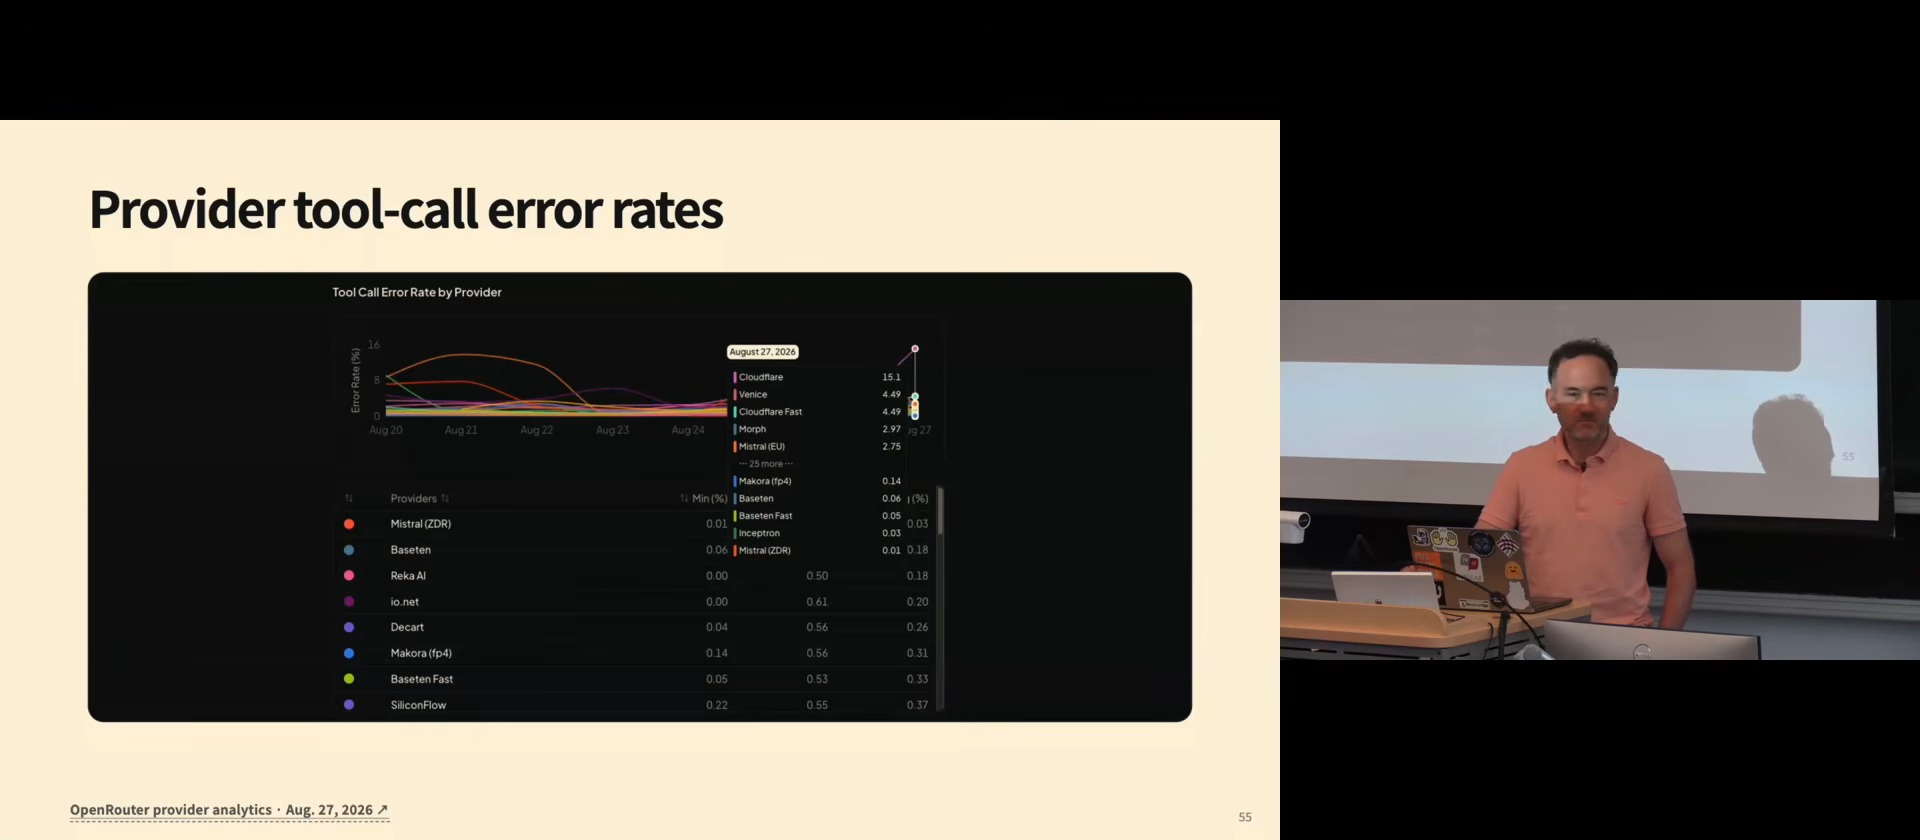
\includegraphics[width=\textwidth]{figures/fig_32_provider_errors.jpg}
\caption{供应商工具调用错误率榜：同一模型的错误率从 0.01\% 级到 15.1\% 级不等\vtag}
\end{figure}
\srcnote{00:52:30--00:52:44}

课上讨论出四类原因，讲者逐条确认：

\begin{itemize}
\item \textbf{量化}：服务商用 FP8 还是 FP4 部署差异很大；讲者的经验是 FP8 级别的工具调用错误明显少于 FP4——后者省成本，但通常更差。
\item \textbf{投机解码}：无损的（lossless）不应改变结果，但有损的会；此时"同一个模型"的说法本身就不成立。
\item \textbf{约束解码是否实现}：有的供应商用自己的推理栈，有的基于 vLLM / SGLang，只有后者默认支持文法约束；不支持的就完全依赖模型自己写对格式。
\item \textbf{服务稳定性}：最无聊但最常见的原因——供应商偶尔不可用，调用直接失败。
\end{itemize}

\begin{warningbox}{把"供应商"当作评测变量}
当你在生产里遇到"同样的提示词，昨天好今天坏"，先怀疑供应商与解码配置，而不是先改提示词。选择模型时同时锁定：模型版本、量化精度、是否开启约束解码、超时与重试策略。这些变量应当写进你的评测报告。
\end{warningbox}

\subsection{本章小结}
工具调用评测要覆盖选择、参数、顺序与端到端执行，并补上效率、可靠性与安全三个运行维度；同一模型在不同供应商之间的差异提醒我们，部署细节与模型本身同等重要。

\section{总结与延伸}

\subsection{讲者的收束}

幻灯片把整讲压成一句话：\textbf{工具使用是一个分层的系统}。

\begin{figure}[H]
\centering
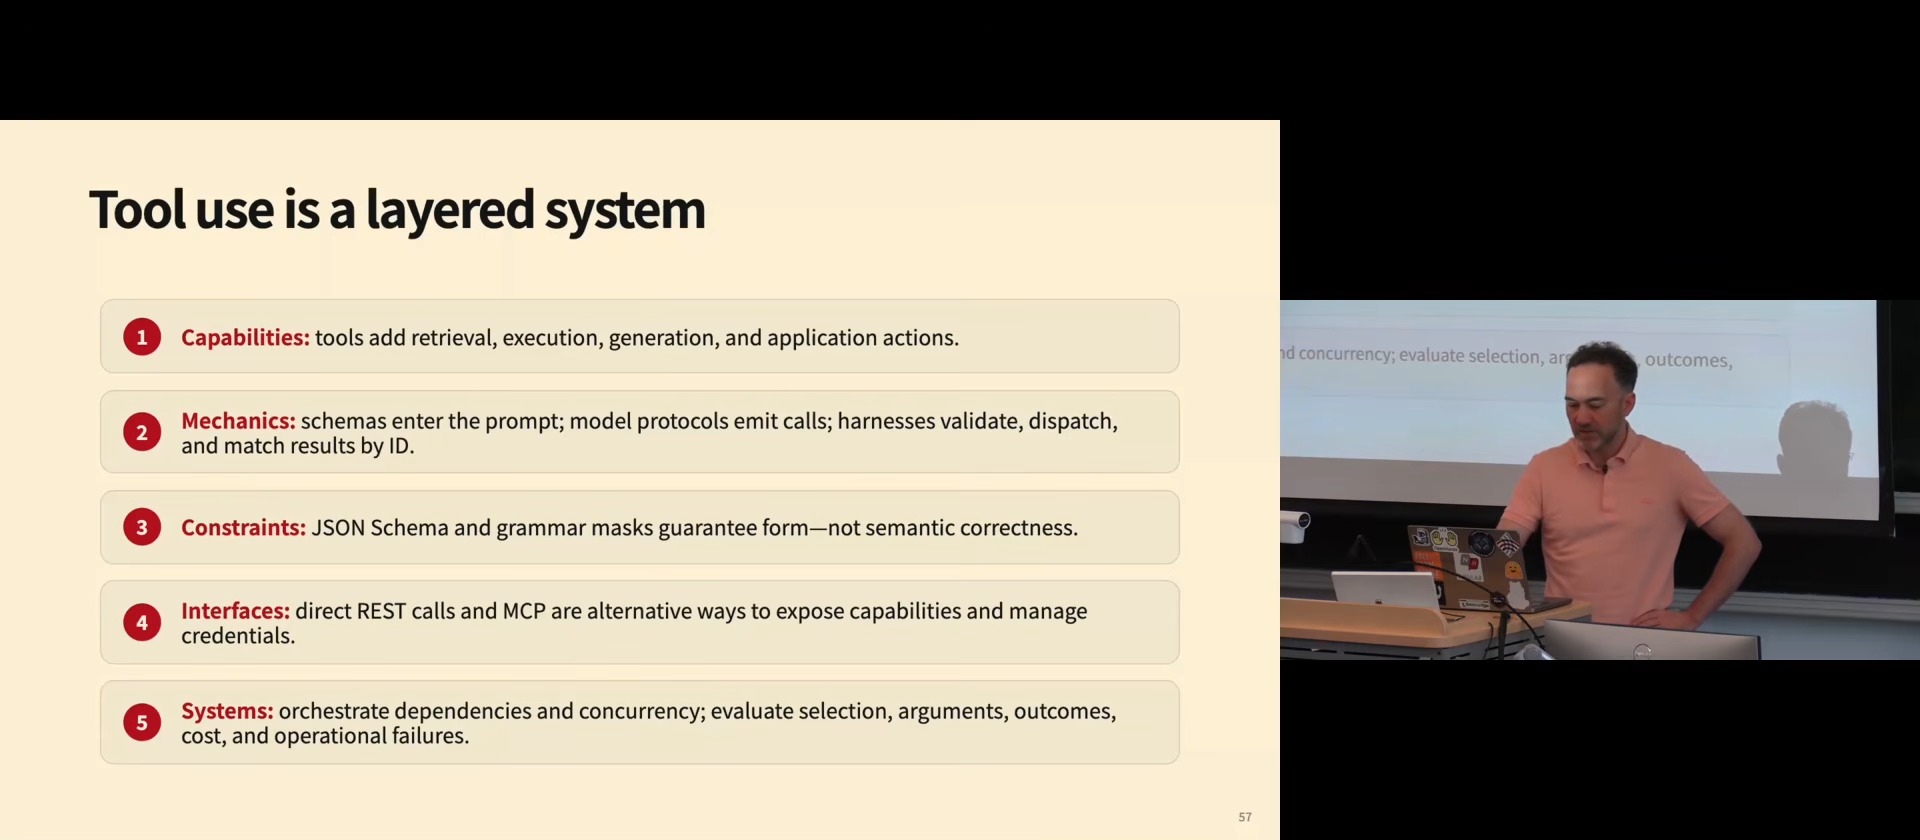
\includegraphics[width=\textwidth]{figures/fig_33_layered.jpg}
\caption{总结：能力层（工具带来检索、执行、生成与应用动作）与机制层（schema 进提示、协议出调用、验证分发、按 ID 配对）\vtag}
\end{figure}
\srcnote{01:00:00--01:00:14}

能力层说的是"工具让 agent 能做什么"：检索、执行、生成与应用。机制层说的是"这件事如何可能"：schema 进入提示、模型按各家协议发出调用、harness 校验并分发、结果按 call ID 配对回填。讲者的提醒同样重要：\textbf{约束只保证形式，不保证语义正确}——一段可以解析的 Python 仍然可能是错的程序。

\subsection{整理者的综合}

把这一讲与第 1 讲接起来，读者可以形成一张完整的"工具调用地图"：

\begin{importantbox}{一页纸的工具调用地图}
\textbf{为什么用}：扩展能力（模型做不到）或促进效率（能做但更贵）——收益必须盖过延迟、成本与风险。\\
\textbf{怎么调}：结构化 JSON 调用与代码化调用两条范式；多步组合优先考虑代码，窄任务优先考虑结构化调用。\\
\textbf{为什么不会写错}：JSON Schema → 上下文无关文法 → 下推自动机 → logits 掩码，把非法 token 的概率清零；唯一例外是 max tokens 截断。\\
\textbf{挂在哪里}：进程内库 / REST（FastAPI + OpenAPI + API key）/ MCP（独立凭证隔离）；共享的是 JSON Schema，不同的是信任边界。\\
\textbf{怎么并行}：只并行互不依赖的调用；收益来自"少生成几轮"；更贵的模型可能因为并行与少走弯路而总成本更低。\\
\textbf{怎么评测}：selection / arguments / order / execution 四层，加上效率、可靠性、安全三个运行维度；供应商与量化同样是变量。
\end{importantbox}

讲者在课程中反复区分事实与判断，本讲也不例外。属于\textbf{事实}的有：畸形调用会导致解析失败、不同模型的协议不同、约束解码能消除格式错误、MCP 的凭证可以分离、供应商之间的错误率差异实测存在。属于\textbf{判断}的有："代码化调用往往更好""更贵的模型可能更便宜""给 agent 的凭证应当即使泄漏也无害"——这些都有具体条件，读者应当结合自己的任务复核。

\subsection{可以继续追问的问题}

\begin{itemize}
\item \textbf{约束解码会不会伤害推理？}掩码把模型限制在合法路径上，但若模型原本想先"想一想"再调用，强约束是否会挤压它的思考空间？
\item \textbf{形式之外还能约束什么？}语法层已经被解决，参数取值、权限与工具选择是否也能用类似的方式在解码期约束（本讲明确说这是不同层次的问题）？
\item \textbf{并行到什么程度？}并行调用省时间，但会放大副作用竞争与失败组合爆炸；合理的并行度如何确定？
\item \textbf{供应商差异如何工程化对抗？}固定版本与量化、自建推理（vLLM/SGLang）、还是多供应商路由加验收测试，哪种组合的性价比最高？
\end{itemize}

\subsection{拓展阅读}
\begin{itemize}
\item \textbf{CodeAct} 类工作（讲者引用的 programmatic tool calling 实证）——代码化调用为什么更有效。
\item \textbf{XGrammar}——约束解码的工程实现，本讲第 4 章的图源。
\item \textbf{Berkeley Function Calling Leaderboard（BFCL V4）}——工具调用评测的公开榜单与数据集。
\item \textbf{Model Context Protocol 规范与官方 registry}——MCP 的发现、传输与认证细节。
\item \textbf{FastAPI / fastMCP 文档}——把函数变成 REST 或 MCP 工具的最短路径。
\end{itemize}

%% --- 正文内容结束 --- %%

\end{document}
